\documentclass[letterpaper,12pt]{report}
\usepackage{tabularx} % extra features for tabular environment
\usepackage{amsmath}  % improve math presentation
\usepackage{amsthm}
\usepackage{tabu}
\newtheorem*{theorem}{Theorem}
\theoremstyle{definition}
\newtheorem{definition}{Definition}[chapter]
\newtheorem{example}{Example}[chapter]
\theoremstyle{remark}
\newtheorem*{remark}{Remark}
\usepackage{caption}
\usepackage{graphicx} % takes care of graphics
\usepackage{tikz}
\usepackage[margin=1in,letterpaper]{geometry} % decreases margins
\usepackage{cite} % takes care of citations
\usepackage[final]{hyperref} % adds hyper links inside the generated pdf file
\hypersetup{
	colorlinks=false,       % false: boxed links; true: colored links
	linkcolor=blue,        % color of internal links
	citecolor=blue,        % color of links to bibliography
	filecolor=magenta,     % color of file links
	urlcolor=blue         
}
\usepackage{amsmath,amssymb}
\DeclareMathOperator{\E}{\textbf{E}}
\DeclareMathOperator{\var}{\text{var}}
\usepackage[T1]{fontenc}

%++++++++++++++++++++++++++++++++++++++++
 
\begin{document}

\title{Mathematics for HFT}
\author{jojo}
\date{June 30, 2020}
\maketitle

\newpage
\vspace*{8cm}
\begin{center}
	\large \emph{
		To Aliza Joshi,\linebreak
		Who loved me when I myself couldn't,\linebreak
		Without her this wouldn't exist.}
\end{center}

\tableofcontents

\part{Basics}
%%%%%%%%%%%%%%%%%%%%%%%%%%%%%%%%%%%%%%%%%%%%%%%%%%%%%%%%%%%%%%%%%%%%
\chapter {Mathematical Induction}
It's simpler to prove recurrence relations using mathematical induction.

Mathematical induction is a general way to prove that some statement about the integer $n$ is true for all $n > n_0$.
\begin{enumerate}
	\item First we prove the statement when $n$ has its smallest value, $n_0$; this is called the basis.
	\item Then we prove the statement for $n > n_0$, assuming that it has already been proved for all values in $ [n_0, n - 1]$, this is called the induction. Such a proof gives infinitely many results with only a finite amount of work.
\end{enumerate}

\textit{Mathematical induction proves that we can climb as high as we like on a ladder, by proving that we can climb onto the bottom rung (the basis) and that from each rung we can climb up to the next one (the induction).}

%%%%%%%%%%%%%%%%%%%%%%%%%%%%%%%%%%%%%%%%%%%%%%%%%%%%%%%%%%%%%%%%%%%%
\chapter {Recurrence Relations}

Loosely speaking, A relation for a quantity (like $T_n$) when defined in terms of the quantity itself (like $T_{n-1}$) constitutes a recurrence relation.

In finding a closed-form expression for a quantity of interest (like $T_n$) we go through three stages:
\begin{enumerate}
    \item Look at small cases. This gives us insight into the problem and helps us
in stages 2 and 3.
    \item Find and prove a mathematical expression for the quantity of interest. This usually requires finding a recurrence relation.
    \item Find and prove a closed form for our mathematical expression.
\end{enumerate}

Sadly nothing can be done for step 1 and 2. But for step 3, we'll discuss few methods.

\section {Repertoire method}
\begin{definition}[Repertoire] A list or supply of dramas, operas, pieces, or parts that a company or person is prepared to perform.
\end{definition}
The repertoire method is a tool to help with the intuitive step of figuring out a closed formula for a recurrence equation. The method works best with recurrences that are ``linear" in the sense that the solutions can be expressed as a sum of arbitrary parameters multiplied by functions of $n$.

\subsection{Motivating example}
Let $a_n=3$ and $b_n=5n^2+1$. Assuming we know the solutions $x_n$ and $y_n$ of the recurrences
\begin{align*}
x_0&=3&y_0&=1\\
x_n&=3+x_{n-1},\quad n>0&y_n&=5n^2+1+y_{n-1},\quad n>0
\end{align*}
then we also know by linearity that the solution of the recurrence
\begin{align*}
z_0&=7\\
z_n&=2n^2+7+z_{n-1}
\end{align*}
is
\begin{align*}
z_n=\frac{11}{5}x_n+\frac{2}{5}y_n
\end{align*}
We observe that in this case we have a repertoire of two solutions $x_n$ and $y_n$ which we can linearly combine in order to find the wanted solution $z_n$. But, we typically start with a recurrence $z_n$ without having a repertoire of proper candidates.

\subsection{Finding solution}
Let's assume we start with a recurrence
\begin{align*}
z_0&=7\\
z_n&=2n^2+7+z_{n-1},\quad n>0\tag{1}
\end{align*}
So, if we try to solve this recurrence by the method of repertoire, we first generalise the recurrence and consider instead

\begin{align*}
\mathcal{Z}_0&=a_0\\
\mathcal{Z}_n&=a_n+\mathcal{Z}_{n-1},\quad n>0
\end{align*}

Now it's time for some creative ideas which is typically the most challenging phase when using this method. We want to find a repertoire consisting of two members. One of them with $a_n=$ const. and the other with $a_n=$ square of n. In order to do so we have to guess some proper candidates for $\mathcal{Z}_n$ which provides us with the wanted $a_n$.

So let's guess a first candidate. This is not too hard (in this case) since setting $\mathcal{Z}_n=n$ gives

\begin{align*}
a_0&=0\\
n&=a_n+n-1\quad n>0
\end{align*}

and we find: $a_0=0$ and $a_n=1,n>0$.

We get the first candidate, let's say $x_n$ with

\begin{align*}
x_0&=0\\
x_n&=1+x_{n-1},\quad n>0\tag{2}
\end{align*}

We can similarly find a proper second candidate which provides us with $a_n=$ square of n by observing that typically the sum of k-th powers of natural numbers is something with a (k+1)-th power. So we guess $\mathcal{Z}_n=n^3$ which gives

\begin{align*}
a_0&=0\\
n^3&=a_n+(n-1)^3\quad n>0
\end{align*}

and we find $a_0=0$ and $a_n=3n^2-3n+1,n>0$.

We get the second candidate, let's say $y_n$ with

\begin{align*}
y_0&=0\\
y_n&=3n^2-3n+1+y_{n-1},\quad n>0\tag{3}
\end{align*}

We observe that $y_n$ also contains a linear term in $n$ which is not wanted, since we need according to (1) $a_n=n^2+7$. So we extend our repertoire by introducing a third member which provides us with $a_n=$ linear term in n. Then we should be able to eliminate the linear term in n by a proper linear combination of the three members. We guess $\mathcal{Z}_n=n^2$ which gives
\begin{align*}
a_0&=0\\
n^2&=a_n+(n-1)^2\quad n>0
\end{align*}
and we find $a_0=0$ and $a_n=2n-1,n>0$.

So we get the third candidate, let's say $u_n$ with

\begin{align*}
u_0&=0\\
u_n&=2n-1+u_{n-1},\quad n>0\tag{4}
\end{align*}

Let's have a look at the repertoire. Overview of the three candidates:
$$
\begin{array}{rlcr}
\mathcal{Z}_n&&a_n&\\
\hline\\
x_n=&n\qquad&1&\qquad\qquad\text{acc. to }(2)\\
y_n=&n^3\qquad&3n^2-3n+1&\qquad\qquad\text{acc. to }(3)\\
u_n=&n^2\qquad&2n-1&\qquad\qquad\text{acc. to }(4)\\
\end{array}
$$
We observe when using an appropriate linear combination
\begin{align*}
a_n&=2n^2+7\\
&=\frac{2}{3}\left(3n^2-3n+1\right)+\left(2n-1\right)+\frac{22}{3}
\end{align*}
and we conclude
\begin{align*}
z_n&=\frac{22}{3}x_n+\frac{2}{3}y_n+u_n+c_0\\
&=\frac{1}{3}n\left(2n^2+3n+22\right)+c_0
\end{align*}

Observe, that we have to determine a constant $c_0$ since we also have to properly respect the initial condition $z_0=7$. We do so by setting $c_0=7$ and so we finally get:
$$z_n=\frac{1}{3}n\left(2n^2+3n+22\right)+7,\quad n\geq 0$$
%%%%%%%%%%%%%%%%%%%%%%%%%%%%%%%%%%%%%%%%%%%%%%%%%%%%%%%%%%%%%
\subsection{Steps}
In order to solve a recurrence of the form
\begin{align*}
x_n=f(n)+g(x_{n-1},x_{n-2},\ldots,x_0)\tag{5}
\end{align*}
\begin{itemize}
    \item we identify building blocks $f_1(n),\ldots,f_k(n)$ of $f(n)$, so that they can be linearly combined in order to form $f(n)$
    \begin{align*}
    f(n)=\lambda_1 f_1(n)+\ldots+\lambda_k f_k(n)
    \end{align*}
    
    \item then we consider the generalised representation of (5) by substituting $f(n)$ with $a_n$.
    \begin{align*}
    \mathcal{Z}_n=a_n+g(\mathcal{Z}_{n-1},\mathcal{Z}_{n-2},\ldots,\mathcal{Z}_0)
    \end{align*}
    
    \item and solve the simpler recurrences
    \begin{align*}
    x_n^{(l)}=f_l(n)+g(x_{n-1},x_{n-2},\ldots,x_0)\quad 1 \leq l \leq k
    \end{align*}
    by proper guessing of $x_n^{(l)}$ in order to get $f_l(n)$.
    
    \item The solutions $x_n^{(l)}$ with $1\leq l \leq k$ form the repertoire of the method in order to solve $x_n$.
    
    \item Determine the linear combination 
    $$f(n)=\lambda_1 f_1(n)+\ldots+\lambda_k f_k(n)$$
    
    \item and deduce the solution
    $$x_n=\lambda_1 x_n^{(1)}+\ldots+\lambda_k x_n^{(k)}+c_0$$
    
    \item Finally determine $c_0$ according to initial conditions
\end{itemize}
\begin{remark} There may be more than one initial condition which are to determine. It may be necessary to extend the repertoire in order to remove unwanted terms which additionally occur during the calculation of the $x_n^{(l)}$.
\end{remark}
%%%%%%%%%%%%%%%%%%%%%%%%%%%%%%%%%%%%%%%%%%%%%%%%%%%%%%%%%%%%%%%
\subsection{More examples}
\subsubsection{Josephus Solution}
Generalised Josephus equations are
\begin{align*}
    f(1) & = \alpha \\
    f(2n) &= 2f(n)+ \beta \\
    f(2n+1) &= 2f(n)+ \gamma 
\end{align*}
Therefore we can write 
$$f(n)=A(n)\alpha+B(n)\beta+C(n)\gamma$$

Using $f(n)=1$
\begin{align*}
    1 &= \alpha \\
    1 &= 2+\beta \\
    1 &= 2+\gamma
\end{align*}
Therefore $(\alpha,\beta,\gamma)=(1,-1,-1)$.

Using $f(n)=n$, we get
\begin{align*}
    1 &=\alpha \\
    2n &= 2n+\beta \\
    2n+1&= 2n+\gamma
\end{align*}
Therefore $(\alpha,\beta,\gamma)=(1,0,1)$.

\emph{Reverse.} Let's consider $(\alpha,\beta,\gamma)=(1,0,0)$. Therefore $f(n)=A(n)$, we get
\begin{align*}
    A(1) &= 1\\
    A(2n)&=2A(n) \\
    A(2n+1)&=2A(n)
\end{align*}
Therefore $A(2^m+l)=2^m, 0 \le l < 2^m$. Combining all three relations, we get
\begin{align*}
    A(n)-B(n)-C(n) &= 1 \\
    A(n)+C(n) &=n\\
    A(n) &= 2^m, \text{where} \; n=2^m+l, 0 \le l < 2^m
\end{align*}
Giving us $f(n) = 2^m \alpha + (2^m-1-l) \beta + l \gamma, \, n=2^m+l, \, 0\le l< 2^m$.

\subsubsection{Summation Recurrence}
Suppose that we have to evaluate $\sum_{k=0}^{n}(a+bk)$. Assuming $\alpha=\beta=a, \gamma=b$, we get
\begin{align*}
    R_0 &= \alpha \\
    R_n &= R_{n-1}+\beta+\gamma n, \quad n>0
\end{align*}
Therefore using different function for $R_n=A(n)\alpha +B(n)\beta+C(n)\gamma$ we get, $R_1=\alpha+\beta+\gamma, \, R_2=\alpha+2\beta+3\gamma$,
\begin{center}
    $$\begin{tabu}{|c|c|c|}\hline
        R_n = 1 & R_n=n & R_n=n^2 \\
        \hline
        \alpha = 1 & \alpha = 0 & \alpha = 0 \\
        \beta = 0  & \beta = 1 &  \beta = -1 \\
        \gamma = 0 & \gamma = 0 & \gamma = 2 \\
        \hline    
    \end{tabu}$$
\end{center}
Thus we have, $A(n)=1, B(n)=n, C(n)=n(n+1)/2$. Since now we have closed form, it is easy to find the original summation.
%%%%%%%%%%%%%%%%%%%%%%%%%%%%%%%%%%%%%%%%%%%%%%%%%%%%%%%%%%
\section{Reducing recurrence to a sum}
Suppose that we have to find $T_n$ in
\begin{align*}
    a_nT_n &= b_nT_{n-1} + c_n \\
\end{align*}
We multiply both sides by a summation factor $s_n$
\begin{align*}
    s_na_nT_n &= s_nb_nT_{n-1} + s_nc_n
\end{align*}
Choose $s_n$ such that $s_nb_n=s_{n-1}a_{n-1}$. Therefore we have
\begin{align*}
    S_n &= s_na_nT_n \quad \text{(suppose)} \\
    S_n &= S_{n-1} + s_nc_n \\
    S_n &= \sum_{k=1}^{n}s_kc_k + s_0a_0T_0 \\
    T_n &= \frac{1}{s_na_n}\left(s_1b_1T_0 + \sum_{k=1}^{n}s_kc_k \right)
\end{align*}
The trick to choose $s_n$ is unfolding its recurrence
$$
s_n = \frac{a_{n-1}a_{n-2}\dots a_{1}}{b_nb_{n-1}\dots b_{2}}
$$
\subsubsection{Example (from \cite{concrete-maths})}
Try to find the $C_n$ in 
\begin{align*}
    C_0 &= 0 \\
    C_n &= n+1 + \frac{2}{n} \sum_{k=0}^{n-1} C_k
\end{align*}
to be the answer (where $H_n$ is the $n^{th}$ harmonic number)
\begin{align*}
    nC_n &= (n+1)C_{n-1}+2n \quad n>0, \quad \text{(hint)} \\
    C_n &= 2(n+1)H_n - 2n
\end{align*}
%%%%%%%%%%%%%%%%%%%%%%%%%%%%%%%%%%%%%%%%%%%%%%%%%%%%%%%%%
\section{Solving Linear Homogeneous Recurrence Relations}
\chapter{Sums}
Discussion on the art of manipulating sums.

\section{Manipulation of Sums}
\subsection{Perturbation Method}
This method allows us to evaluate sums in closed form and starts by knocking of first and last terms in a sum and trying to co-relate the new sum.

\subsubsection{Example}
Suppose that $S_n = \sum_{0 \le k \le n}k\,2^k$. Now adding last term to the sum, we get
\begin{align*}
S_n + (n+1)2^{n+1} &= \sum_{0\le k \le n}k\,2^k + (n+1)2^{n+1} \\
    &= 02^0 + \sum_{1 \le k \le n+1}k\,2^k \quad \text{(knock first term)}\\
    &= \sum_{1 \le k+1 \le n+1} (k+1)2^{k+1} \\
    &= 2 \left(2^{n+2}-2 + \sum_{0\le k \le n} k2^k \right) \\
    &= 2 \left(2^{n+2}-2+S_n \right)\\
\end{align*}
Finally we get $S_n = (n-1)2^{n+1}+2$.

\subsection{Differentiate both sides}
Useful for summations like $\sum kx^k$,
\begin{align*}
    \sum_{k=0}^n kx^k &= x \frac{d}{dx}\left(\sum_{k=0}^nx^k\right) \\
    &= x \frac{d}{dx}\left(\frac{1-x^{k+1}}{1-x}\right)
\end{align*}
\part {Number Theory}
\part {Combinatorics}
\part {Probability}
\chapter{Sample Space and Probability}
Our main objective of this section is to develop the art of describing un­certainty in terms of probabilistic models, as  well as the skill of probabilistic reasoning. The first step, which is the subject of this chapter, is to describe the generic structure of such models and their basic properties. The models we consider assign probabilities to collections (sets) of possible outcomes.

\section{Probabilistic Models}

A probabilistic model is a mathematical description of an uncertain situation. It's elements are:

\begin{enumerate}
    \item \textbf{Sample space:} The set of all possible outcomes.
    \item \textbf{Probability law:} It assign to a set $A$ of possible outcomes (also called an \textbf{event}) a non-negative number $\Pr(A)$ called as the probability of $A$. It encodes our belief of the likelihood of the event. It must satisfy properties described below.
\end{enumerate}

\subsection{Terminologies}

\begin{itemize}
    \item Every probability model involves an underlying process called the experiment.
    \item An experiment produces exactly one of the several possible outcomes.
    \item The set of \textit{all} possible outcomes is called sample space. The outcomes in this set are mutually exclusive and collectively exhaustive.
    \item A subset of sample space (collection of possible outcomes) is called an event.
\end{itemize}

\subsection{Probability Laws}
The probability law assigns to  every event $A$, a number $\Pr(A)$, called the probability of $A$, satisfying the following axioms.

\begin{enumerate}
    \item \textbf{Non-negativity:} $\Pr(A)\ge 0$ for every $A$.
    \item \textbf{Additivity:} If $A$ and $B$ are two disjoint events then the probability of their union satisfies $\Pr(A \cup B)=\Pr(A)+\Pr(B)$.
    \item \textbf{Normalization:} $\Pr(\Omega)=1$
    \item \textbf{Discrete Probability Law:} If the sample space consists of a finite number of possible outcomes, then the probability law is specified by the  probabilities of the events that consist of a single element.  In particular, the probability of any event $\{s_1, s_2, \dots, s_n\}$ is the sum of the probabilities of its elements:
    \[ \Pr(\{s_1, s_2, \dots, s_n\}) = \Pr(\{s_1\}) + \dots + \Pr(\{s_n \}) \]
\end{enumerate}

\subsection{Models and Reality}
The framework of probability theory can be  used to  analyze uncertainty in  a wide variety of physical contexts. Typically, this involves two distinct stages. 
\begin{enumerate}
    \item \textit{(Connect real world to mathematics)} We  construct a probabilistic model by specifying a prob­ability  law on a suitably defined  sample space. There are no hard rules to guide this step, other than  the  requirement that the probability law con­form to the three axioms. Reasonable people may disagree on which model best represents reality. In many cases, one may even want to use a some­what "incorrect"  model, if it is simpler than  the "correct" one or allows for tractable calculations. This is consistent with common practice in science where the choice of model is a tradeoff between accuracy and simplicity/tractability.
    \item \textit{(Working with model)} We now work with the fully specified probabilistic model and deduce the probabilities of the interesting events. This step is regulated by the rules of logic and all conceivable questions have precise answers. Sometimes it would be difficult to carry out the calculations but there's no room for ambiguity.
\end{enumerate}

\section{Conditional Probability}
Way to reason about outcome of an experiment based on partial information. In more precise terms, given an experiment, a corresponding sample space, and a probability law, suppose that we know  that the outcome is within some given event $B$. We wish to quantify the likelihood that  the outcome also belongs to some other  given event $A$. We thus  seek to construct a  new probability law that takes into account the available knowledge: a probability law that for any event $A$, specifies conditional probability of $A$ given $B$, denoted by $\Pr(A|B)$.

\[\boxed{\Pr(A|B)=\frac{\Pr(A \cap B)}{\Pr(B)} }\]

\subsection{Conditional Probabilities Specify a Probability Law}
\begin{enumerate}
    \item Non-negativity is clear.
    \item Additivity: Suppose $A_1$ and $A_2$ are two disjoint events.
            \[\Pr(A_1 \cup A_2|B)=\frac{\Pr(A_1 \cap B)\cup \Pr(A_2 \cap B)}{\Pr(B)}=\frac{\Pr(A_1 \cap B)+\Pr(A_2\cap B)}{\Pr(B)}=\Pr(A_1|B)+\Pr(A_2|B)\]
    \item Normalization: \[\Pr(\Omega | B)=\frac{\Pr(\Omega \cup B)}{\Pr(B)}=\frac{\Pr(B)}{\Pr(B)}=1\]
\end{enumerate}

\subsection{Properties of Conditional Probability}
\begin{itemize}
    \item The conditional probabilities specifies a new (conditional) probability law on the same sample space $\Omega$. In particular, all the probability laws remains valid for conditional probability laws.
    \item Conditional probabilities can also be viewed as a probability law on a new universe $B$, because all of the conditional probability is concentrated on $B$.
\end{itemize}

\subsection{Using Conditional Probability for Modeling}
When constructing probabilistic models for experiments that have a sequential character, it is often natural and convenient to first specify conditional prob­abilities and then use them to determine unconditional probabilities.

Remember the radar and the aeroplane detection example.

Rules for calculating probabilities in conjunction with a tree-based sequential description of an experiment are:

\begin{enumerate}
    \item Set up the tree so that an event of interest is associated with a leaf. We view the occurrence of the event as a sequence of steps, namely, the traversals of the branches along the path from root to the leaf.
    \item We record the conditional probabilities associated with the branches of the tree.
    \item We obtain the probability of a leaf by multiplying the probabilities recorded along the corresponding path of the tree.
\end{enumerate}
\subsubsection{Multiplication Rule}
We use the following rule to find the probability of a leaf by multiplying the probabilities along the edges.
\[\boxed{\Pr(\cap_{i=1}^{n}A_i)=\Pr(A_1)\Pr(A_2|A_1)\Pr(A_3|A_2\cap A_1)\cdots \Pr(A_n|\cap_{i=1}^{n-1}A_i)}\]

\subsubsection{Example}
There are 4 graduate students and 12 undergraduate students to be divided into groups of 4 with 4 students each. Find the probability that each group has a graduate student.

Answer: First place the first graduate student then sequentially place other graduate students in a different group than the previously assigned groups of graduate students. Thus multiplication rule can be used.
\[\frac{16}{16} \times \frac{12}{15} \times \frac{8}{14} \times \frac{4}{13} \]

\section{Total Probability and Bayes' Rule}
Let $A_1,\dots,A_n$ be disjoint events that form a partition of the sample space (any outcome belongs to exactly one of the event $A_1,\dots,A_n$). Then for any event $B$,
\begin{align*}
    \Pr(B) &= \Pr(A_1 \cap B) + \cdots + \Pr(A_n \cap B)  \\
     &=  \Pr(A_1)\Pr(B|A_1) + \cdots + \Pr(A_n)\Pr(B|A_n)
\end{align*}

Probability of $B$ can also be visualized as the weighted average of the partitions.

\subsection{Inference and Bayes' Rule}

\subsubsection{Bayes' Rule}
Let $A_1,\dots,A_n$ be disjoint events that form a partition of the sample space. Then for any event $B, \; \Pr(B)>0$, we have,

\begin{align*}
    \Pr(A_i|B) &= \frac{\Pr(A_i)\Pr(B|A_i)}{\Pr(B)} \\
             &= \frac{\Pr(A_i)\Pr(B|A_i)}{\Pr(A_1)\Pr(B|A_1) + \cdots + \Pr(A_n)\Pr(B|A_n)}
\end{align*}

This equation is used for cause-effect models. Assume that for every cause we have the probability of the effect. This corresponds to the cause to effect direction. 
\[\text{Cause} \iff \text{Effect}\]

Given that the effect is observed, what is the probability that it is caused by a specific cause. This is the effect to cause direction and also called as inference.

\section{Independence}
$\Pr(A|B)$ captures the partial information that event $B$ provides about $A$. If $B$ does not provide any information about $A$, then 
\[\Pr(A|B) = \Pr(A), \quad \quad \Pr(B)>0\]
The above definition requires that $\Pr(B)>0$ which is not general, so instead the following definition is generally used
\[\boxed{\Pr(A \cap B)  =\Pr(A)\Pr(B)}\]
We say that $A$ and $B$ are independent.

\subsection{Conditional Independence}
Since conditional probabilities are no different than "normal" probabilities as they also form a legitimate probability law we can condition on an event with a minor change in the formula.
Given an event $C$, two events $A$, $B$ are conditionally independent if,
\[ \boxed{\Pr(A \cap B|C)=\Pr(A|C)\Pr(B|C)}\]
or
\[\Pr(A |B \cap C)=\Pr(A|B)\]

In second equation, this relation states that if $C$ is known to have occurred, the additional knowledge that $B$ also occurred does not change the probability of $A$.

Interestingly, independence of two events $A$ and $B$ with respect to  the unconditional probability law, does not imply conditional independence, and vice versa.

\subsection{Independence of Several Events}

We say that the events $A_1, \dots, A_n$, are independent if

\[\boxed{\Pr\left(\bigcap_{i \in S} A_i\right)=\prod_{i \in S}\Pr(A_i), \quad \text{for every subset S of} \; \{1, 2, \dots, n\} }\]

Important remarks:
\begin{itemize}
    \item Pairwise independence does not imply Independence.
    \item The equality $\Pr(A_1 \cap A_2 \cap A_3)=\Pr(A_1)\Pr(A_2)\Pr(A_3)$ is not enough for Independence.
\end{itemize}


\newcommand{\RV}{Random Variable } 
\newcommand{\rv}{random variable } 
\chapter{Discrete \RV}

\section{Basic Concepts}
Given an experiment and a set of possible outcomes (sample space), a \rv associates a particular number with each outcome. Thus, \textbf{ a \RV is just a function from outcomes to $\Re$}. The associated numerical value is simply called as the value of the \rv.

\begin{figure}[h]
   \center
   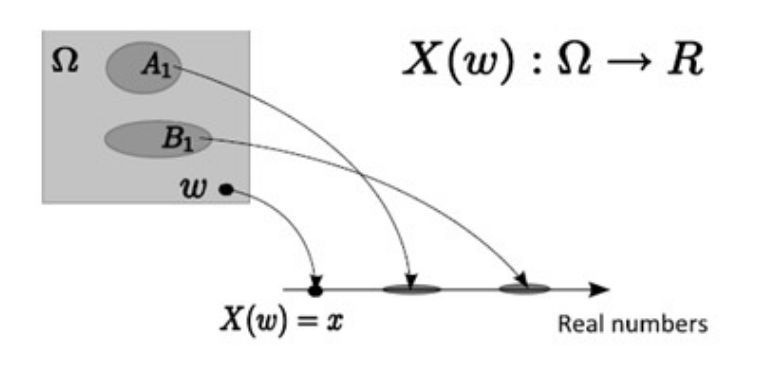
\includegraphics[width=.6\textwidth]{images/P_random_variable.jpg}
   \captionsetup{width=0.7\textwidth}
   \caption{Visualization of a \RV as a mapping from outcomes to a numerical value}
\end{figure}

\begin{definition}
    A \rv is a real-valued function of the outcome of the experiment.
\end{definition}

\subsection{Main concepts related to \rv}
Starting with a probabilistic model of an experiment:
\begin{itemize}
    \item A function of a \rv defines another random variable.
    \item A \rv can be associated with certain \textit{averages} of interest: mean and variance.
    \item A \rv can be conditioned on an event or another random variable.
    \item Notion of independence of a \rv with another \rv or an event.
\end{itemize}

\begin{definition}
    A \rv is called \textbf{discrete} if the set of values that it takes is finite or countably infinite.
\end{definition}

\subsection{Concepts related to Discrete \RV}
Starting with a probabilistic model of an experiment:
\begin{itemize}
    \item A discrete \rv has an associated probability mass function (PMF) which gives the probability of each numerical value that the \rv can take.
    \item A function of a discrete \rv defines another discrete \rv whose PMF can be obtained from the PMF of the original random variable.
\end{itemize}

This chapter will only exercise notation of the concepts that we've already studied previously (conditioning, independence, etc.) and the only new concept will be the mean and the variances.

\section {Probability Mass Function}
A PMF for a \rv $X$, is denoted by $p_X(x)$ is the probability of the event $\{X=x\}$, consisting of all outcomes that give rise to a value of $X$ equal to $x$:
\[p_X(x)=P(\{X=x\})\]

We'll avoid writing braces for brevity and use upper case characters for \RV and lower case characters for the values that the \rv can take.

We have $\sum_x p_X(x)=1$, where $x$ ranges for all values of the \rv $X$. Similarly for any set $S$ of possible values of $X$ 
\[P(X \in S) = \sum_{x\in S} p_X(x)\].

\subsection{Calculation of PMF of a \RV $X$}
For each possible values $x$ of $X$
\begin{enumerate}
    \item Collect all possible outcomes that give rise to event $\{X=x\}$
    \item Add their probabilities to obtain $p_X(x)$
\end{enumerate}

\section{Functions of a \RV}
If $Y=g(X)$ is a function of a rv $X$, then $Y$ is also a \rv since it provides a numerical value for each possible outcome. If $X$ is a discrete \rv then $Y$ is also a discrete \rv and its PMF can be calculated using PMF of $X$. 

In particular, to obtain $p_Y(y)$ for any $y$, we add the probabilities of all values $x$ such that $g(x)=y$
\[p_Y(y)=\sum_{x|g(x)=y}p_X(x)\]

\section{Expectation, Mean, Variance}
\subsection{Expectation}
\begin{definition}
    The expected value (also called as mean or expectation) of a \rv X with PMF $p_X(x)$ is 
    \[ \boxed{\E[X] = \sum_x x \, p_X(x)}\]
\end{definition}

Expectation can be thought of as a weighted average of all possible values of a \rv $X$. Analogously expected value corresponds to the \textit{centre of gravity} of the PMF.

\subsection{Variance, Moments and the Expected Value Rule}
We define the $n^{th}$ moment as $\E[X^n]$, the expected value of the \rv $X^n$. The first moment is just the mean.

Another interesting quantity is variance which is denoted by var($X$) and is defined as the expected value of $(X-\E[X])^2$, i.e.,
\[\text{var}(X) = \E[(X-\E[X])^2]\]
The variance is the measure of dispersion of $X$ around its mean. Another measure is standard deviation which is defined as the square root of the variance and is denoted by 
\[\sigma_X = \sqrt{\text{var}(X)}\]

\subsubsection{Expected Value Rule for Function of \RV}
Let $X$ be a \rv and let $g(X)$ be a function of $X$. Then the expected value of the \rv $g(X)$ is
\[\E[g(X)] = \sum_x g(x) p_X(x)\]

This allows us to avoid calculating the PMF of $g(X)$ and use the PMF of the original \rv

Using the above rule var($X$) is

\[\text{var}(X) = \sum_x (x-\E[X])^2 p_X(x)\]
Similarly, the $n^{th}$ moment is
$\E[X^n]=\sum_x x^n \, p_X(x)$

\subsection{Properties of Mean and Variance}
Let $X$ be a \rv and suppose $Y=aX+b$, where $a$, $b$ are given scalers. Then,
\[\boxed{\E[Y] = a\E[X]+b}\]
\[\boxed{\text{var}(Y) = a^2 \, \text{var}(X)}\]

Variance can also be written as
\[\boxed{\text{var}(X) = \E[X^2] - \E[X]^2}\]

\begin{remark}
    Unless $g(X)$ is a linear function it is not generally true that $\E[g(X)]$ is equal to $g(\E[X])$.
\end{remark}

\section{Joint PMFs of Multiple \RV}
Probability models generally involve multiple random variables. For example for a medical diagnosis, multiple tests may be significant. All of the \rv are associated with the same experiment, same sample space, same probability law and their values can relate in interesting ways.

For two \rv $X$ and $Y$ the joint probability that $\{X=x, Y=y\}$ is captured by $p_{X,Y}(x,y)$
\begin{align*}
    p_{X,Y}(x,y) &= P(\{X=x\} \cap \{Y=y\}) \\
                 &= P(X=x, Y=y)
\end{align*}

Using Joint PMF the probability for an event $A$ that consists of some pairs $(x,y)$ is given by

\[P((X,Y)\in A) = \sum_{(x,y)\in A}p_{X,Y}(x, y)\]

In fact we calculate the marginal PMF of $X$ and $Y$ as
\begin{align*}
    p_X(x) &= \sum_y p_{X,Y}(x, y) \\
    p_Y(y) &= \sum_x p_{X,Y}(x, y)
\end{align*}

The easy way to compute marginal probabilities is to use tabular method. In this case the Joint PMF is laid in a form of table and the marginal PMF for a given $x$ or $y$ can be found by summing the value of Joint PMF along the axis of $x$ or $y$.

\subsection{Functions of Multiple \RV}
Suppose that $Z=g(X, Y)$ be a random variable then the PMF of $Z$ is given by
\[p_Z(z)= \sum_{(x,y)|g(x,y)=z}p_{X,Y}(x,y)\]
Furthermore the expected value naturally extends and takes the from
\[\E[g(X,Y)] = \sum_x \sum_y g(x,y)p_{X,Y}(x,y)\]

If $g$ is linear and takes the form $aX+bY+c$ then the expected value is
\[\E[aX+bY+c]=a\E[X]+b\E[Y]+c\]

\begin{remark}
    The process can be extended to make it work for more than two \rv analogously.
\end{remark}

\subsubsection{Example: The Hat Problem}
Suppose that $n$ gentlemen picks up the hat randomly one by one from the pool of hats after a party. What is the expected value of the number of person getting their own hat back?

Answer: We introduce \textbf{indicator \rv} $X_i$ which denotes that the $i^{th}$ person got his own hat back. $X_i=1$ if the person got his own hat back and 0 otherwise. Therefore $P(X_i=1)=1/n$ and $P(X_i=0)=1-1/n$. The mean is therefore,
\[\E[X_i]=1 \cdot \frac{1}{n}+0 \cdot \frac{n-1}{n} = \frac{1}{n}\]
We have
\begin{align*}
    X &= X_1 + X_2 + \cdots + X_n \\
    \E[X] &= \E[X_1] + \E[X_2] + \cdots + \E[X_n] \\
         &= n \cdot \frac{1}{n} = 1
\end{align*} \qed

\section{Conditioning}
We introduce the conditional PMF given a certain event or given the value of another \rv so therefore there wouldn't be any new concepts.

\subsection{Conditioning a \RV on an Event}
The conditional PMF of a \rv conditioned on an event $A$ with $P(A)>0$ is defined by
\[p_{X|A}(x)=P(X=x|A)=\frac{P(\{X=x\}\cap A)}{P(A)}\]

Also we have the following relations

\begin{align*}
    P(A) &= \sum_x P(\{X=x\} \cap A) \\
     &= \sum_x p_{X|A}(x)    = 1
\end{align*}
This is because the events $\{X=x\} \cap A$ are disjoint for different values of $x$ and their union is $A$.

\begin{remark}
    Thus $p_{X|A}$ is a legitimate PMF.
\end{remark}

The conditional PMF is obtained the same way as the unconditional counterpart. Add all the probabilities of events that give rise to both the events $\{X=x\}$ and $A$. Then normalize by dividing with $P(A)$.

\begin{figure}[h]
    \center
    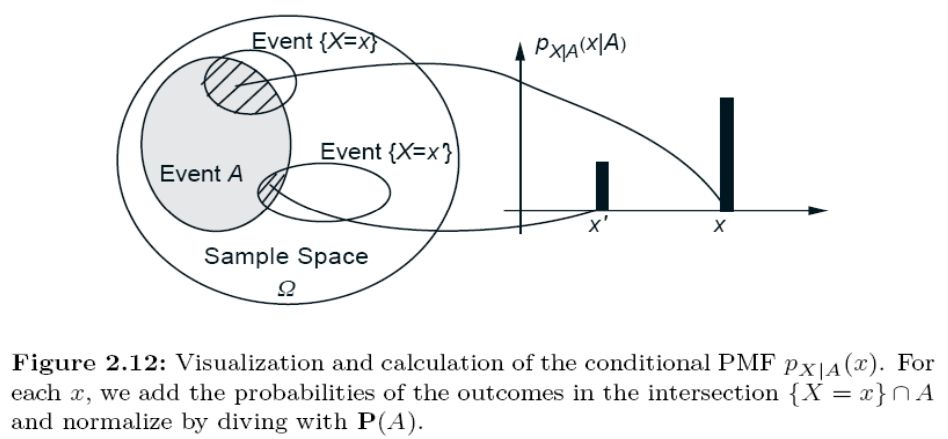
\includegraphics[width=.7\textwidth]{images/P_conditional_pmf.jpg}
 \end{figure}

 \subsection{Conditioning one \RV on another}
 If we are given that out of the two \rv $X$ and $Y$ that $Y=y$ has occurred with probability $p_Y(y)>0$ then it gives us partial knowledge about the value of $X$. This knowledge is captured by conditional PMF $p_{X|Y}$ of $X$ given $Y$, which is defined by the definition of $p_{X|A}$ to the events $A$ of the form $\{Y=y\}$
 \[p_{X|Y}(x|y)= P(X=x|Y=y)\]

 According to the definition of conditional probabilities
 \[p_{X|Y}(x|y)=\frac{P(X=x,Y=y)}{P(Y=y)} = \frac{p_{X,Y}(x,y)}{p_Y(y)}\]

 Fixing some $Y=y$, consider $p_{X|Y}(x|y)$ as a function of $x$. This function is a valid PMF for $X$ as it assigns a non-negative value for each outcome and these values add up to 1.

 The shape of $p_{X|Y}$ is similar to $p_{X,Y}$  except that it is divided by $p_Y(y)$ which enforces the normalization property ($\sum_x p_{X|Y}(x|y)=1$).

 We also have \[p_{X,Y}(x,y)=p_Y(y) p_{X|Y}(x|y) =p_X(x) p_{Y|X}(y|x)\]

 Conditional PMFs can be used to calculate marignal PMFs
 \[p_X(x)=\sum_y p_{X,Y}(x,y)=\sum_y p_Y(y)p_{X|Y}(x|y)\]

 This provides a divide and conquer method for calculating marignal PMFs and is similar in spirit to total probability theorum.

 If $A_1, \ldots, A_n$ are disjoint events that form a partition of the sample space ($P(A_i)>0$ for all $i$) then
 \[p_X(x)=\sum_{i=1}^{n} P(A_i) p_{X|A_i}(x)\]

 This is a special case of total probability theorum. Furthermore for any event $B$ with $P(A_i \cap B)>0$ for all $i$ then
 \[p_{X|B}(x)=\sum_{i=1}^n P(A_i|B)p_{X|A_i \cap B}(x)\]

 \subsection{Conditional Expectation}
 A conditional PMF can be thought of as an ordinary PMF over a new universe determined by the conditioning event. In the same spirit, a conditional expectation is the ordinary expectation except that it refers to the new universe, and all the probabilities and PMFs are replaced by their conditional counterparts.

 If $X$ and $Y$ are the two \rv associated with the same experiment
 \begin{enumerate}
     \item The conditional expectation of $X$ given an event $A$ with $P(A)>0$ is defined by
        \[\E[X|A]=\sum_x xp_{X|A}(x)\]
     for a function $g(X)$ we have
        \[\E[g(X)|A]=\sum_x g(x) p_{X|A}(x)\]
     \item The conditional expectation of $X$ that $Y$ takes a given $y$ is 
        \[\E[X|Y=y]=\sum_x x p_{X|Y}(x|y)\]
     \item If $A_1, \ldots, A_n$ be disjoint events that form a partition of the sample space ($P(A_i)>0$ for all $i$) then
        \[\E[X]=\sum_{i=1}^n P(A_i) \E[X|A_i]\]
    Furthermore for any event $B$ with $P(A_i \cap B)>0$ for all $i$ then
        \[\E[X|B]=\sum_{i=1}^n P(A_i|B)\E[X|A_i \cap B]\]
    \item We have \[\E[X]=\sum_y p_Y(y) \E[X|Y=y]\]
    \end{enumerate}

Last 3 equalities are equivalent and are therefore termed collectively as \textbf{total expectation theorum}. They all follow the idea that "The unconditional average can be obtained by averaging the conditional averages."

\subsubsection{Example: Geometric Mean and Variance}
Suppose that $X$ is a geometric \rv with PMF
\[p_X(k)=(1-p)^{k-1}p, \quad k=1,2,\ldots\]
The mean and variance is given by
\begin{align*}
    \E[X] &= \sum_{k=1}^{\infty} k (1-p)^{k-1} p \\
    \text{var}(X) &= \sum_{k=1}^{\infty}(k-\E[X])^2(1-p)^{k-1}p
\end{align*}
This is tedious to calculate. Let's think simpler.

If the first try is successful then we have $X=1$ and $\E[X|X=1]=1$. Otherwise we have wasted a trial and we are back at the same problem to be solved. Thus $\E[X|X>1]=1+\E[X]$.
Therefore 
\begin{align*}
    \E[X] &= P(X=1)\E[X|X=1] + P(X>1)(1+\E[X]) \\
         &= p + (1-p)(1+\E[X]) = \frac{1}{p} \\
\end{align*}

With a similar reasoning we have
\begin{align*}
    \E[X^2|X=1] &= 1 \\
    \E[X^2|X>1] &= \E[(1+X)^2] = 1 + 2\E[X]+\E[X^2] \\
    \E[X^2] &= p \cdot 1 + (1-p)(1+2\E[X]+\E[X^2]) \\
           &= \frac{1+2(1-p)\E[X]}{p} = \frac{2-p}{p^2} \\
    \text{var}(X)&= \E[X^2]-\E[X]^2=\frac{1-p}{p^2}
\end{align*}
\qed
\subsubsection{Example: Two Envelopes Paradox.}
See Example 2.18 (p. 106) \cite{intro-to-prob} if you're curious.

\section{Independence}
The concepts in this section will be analogous to the concepts of independence between events. They are developed by simply introducing suitable events involving the possible values of the random variable and by considering the independence of these events.

\subsection{Independence of a \RV from an Event}
Intuitively this means that the occurrence of an event provides does not provide any extra information on the likeliness of the different values that the \rv can take.

We say that a \rv is independent of an event $A$ if 
\[\boxed{P(X=x \text{ and } A)=P(X=x)P(A)=p_X(x)P(A)=p_{X|A}(x)P(A)} \qquad \forall x\]

This implies that for every value that the \rv can take the above equality must hold. As long as $P(A)>0$, independence is same as the condition
\[ \boxed{p_{X|A}(x) = p_X(x)} \qquad \forall x\]

\subsection{Independence of \RV}
We say that two \rv are independent if
\[\boxed{p_{X,Y}=p_X(x)p_Y(y)} \qquad \forall x,y\]

In case of conditioning event $A$ we have a new universe and the PMFs have to be replaced by the conditional counterparts. $X, Y$ are said to be conditionally independent given an positive probability event $A$, if

\[\boxed{P(X=x, Y=y | A) = p_{X|A}(x) p_{Y|A}(y)} \qquad \forall x,y\]

This is equivalent to 
\[p_{X|Y,A}(x|y)=p_{X|A}(x) \qquad \forall x,y \text{ such that } p_{Y|A}(y)>0\]

\begin{remark}
    In case of events conditional independence may not imply unconditional independence and vice versa.
\end{remark}

If two $X, Y$ are independent then 
\[\E[XY]=\E[X]\E[Y]\] 
\[ \boxed{\E[g(X)h(Y)]=\E[g(x)]\E[h(Y)]}\]

We have
\begin{center}
    var($X+Y$) = var($X$) $+$ var($Y$) \\
    var($X_1+\cdots+X_n$) = var($X_1$) $+ \cdots+$ var($X_n$) 
\end{center}

\subsection{Independence of several \RV}
Independence of several variables is a simple extension to the above discussion. If for $X, Y, Z$ the following condition holds
\[p_{X,Y,Z}=p_X(x)p_Y(y)p_Z(z)  \qquad \forall x,y,z\]
then the random variables are independent.

\chapter{General \RV}
The \rv used in this chapter takes a continuous range of possible values. There is a striking similarity between techniques used to manipulate discrete and continuous \rv.

\section{Continous \rv and PDFs}
A \rv $X$ is called continuous if there is a \textit{non-negative} function $f_X$ called the probability density function of $X$, or PDF, such that
\[\boxed { P(X\in B) = \int_B f_X(x) dx }\]
for every subset $B$ of real line. The probability that $X$ falls within the interval $[a,b]$ is
\[P(a \le X \le b) = \int_a^b f_X(x) dx\]
can be interpreted as the area under the graph of the PDF (see Fig. 3.1).

\begin{figure}[h]
    \center
    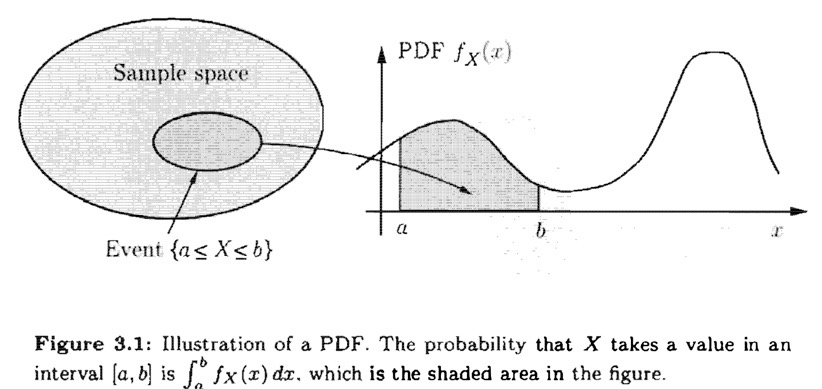
\includegraphics[width=.8\textwidth]{images/P_pdf.jpeg}
 \end{figure}

 For a single value $a$, we have $P(X=a)=\int_a^a f_X(x) dx = 0$. For this reason including or excluding the end points of an interval has no effect on its probability.

 \subsection{Interpretation of PDFs}
 Note that for small intervals $[x,x+\delta]$, we have
 \[P([x,x+\delta]) = \int_x^{x+\delta} f_X(t)dt \approx f_X(x) \cdot \delta\]

 We can view PDFs as the "probability mass per unit length" near $x$ (see Fig. 3.2). 

 Although PDFs are used to calculate the event probabilities, $f_X(x)$ is not the probability of any particular event. In particular, it is not restricted to be less than or equal to one.

 \begin{figure}[h]
    \center
    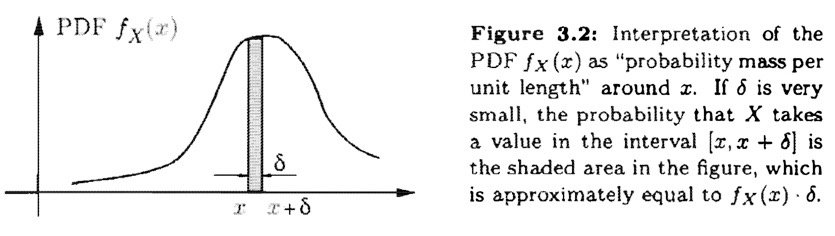
\includegraphics[width=.8\textwidth]{images/P_pdf_interpret.jpeg}
 \end{figure}

 \subsubsection{Example: PDF can take arbitrarily large values.}
 Consider  a \rv $X$ with PDF
 \[f_X(x) = \begin{cases}
     \frac{1}{2\sqrt{x}} & 0 < x \le 1 \\
     0 & \text{otherwise}
 \end{cases}\]

 This is still a valid PDF even when $f_X(x)$ becomes infinitely large as $x$ approaches zero because
 \[\int_{-\infty}^{+\infty}f_X(x) dx = \int_0^1 \frac{1}{2\sqrt{x}} dx = \sqrt{x}\Bigr|_0^1 = 1\] \qed

 \subsection{Properties of a PDF}
 \begin{enumerate}
     \item The function $f_X$ must be non-negative, i.e., $f_X(x) \ge 0$ for all $x$.
     \item For any subset $B$ of real line,
     \[P(X \in B) = \int_B f_X(x) dx\]
     \item The normalization property must hold
     \[\int_{-\infty}^{+\infty}f_X(x) dx=P(-\infty < X < +\infty) = 1\]
     This means that the area under the PDF must integrate to 1.
     \item If $\delta$ is very small, then $P([x,x+\delta]) \approx f_X(x) \cdot \delta$
 \end{enumerate}

 \subsection{Expectation}
 The expected value or mean of a continuous \rv $X$ is defined by
 \[ \boxed{\E [X] = \int_{-\infty}^{+\infty}xf_X(x) \; dx }\]

 This is similar to the discrete case except that 
 \begin{enumerate}
    \item PMF is replaced by the PDF.
    \item The summation is replaced by the integral.
 \end{enumerate}

 $\E[X]$ can be interpreted as the "center of gravity" of the PDF and also as the anticipated average value of $X$ over a large number of independent trails of the experiment. Its mathematical property is same as the discrete case --- after all the integral is just a limiting form of a sum.

 If $X$ is a continuous \rv with PDF $f_X(x)$ then $g(X)$ can be either a continuous or discrete \rv with the following properties
 \begin{itemize}
     \item Expected value is given by
     \[\E[g(X)]=\int_{-\infty}^{+\infty}g(x)f_X(x) \; dx\]
     \item The variance of $X$ is defined by
     \[\text{var}(X)=\E[(X-\E[X])^2]=\int_{-\infty}^{+\infty}(x-\E[x])^2 f_X(x) \; dx\]
     \item We have
     \[0 \le \text{var}(X)=\E[X^2]-\E[X]^2\]
     \item If $Y=aX+b$, where $a$ and $b$ are scalars, then
     \[\E[Y]=a\E[X]+b, \qquad \text{var}(Y)=a^2\text{var}(X)\]
 \end{itemize}

 \section{Cumulative Distribution Functions}
 CDFs provides a unified mathematical concept to deal with PMFs in discrete case and PDFs in continuous case. It helps to abstract the nature of the random variable.

 The CDF for a \rv is denoted by $F_X(x)$ and is the probability $P(X \le x)$. In particular, for every $x$ we have
 \[\boxed{
     F_X(x)=P(X \le x) = \begin{cases}
         \sum_{k \le x}p_X(k) & X \text{ is discrete} \\
         \int_{-\infty}^{x}f_X(t) \; dt & X \text{ is continuous}
     \end{cases}
 }\]
 
 Since $\{X\le x \}$ is always an event and has a well defined probability and therefore any unambiguous specification of the probabilities of all events of the same form (through PMF, PDF or CDF) will be referred as the probability law of the \rv $X$.

 \subsection{Properties of CDF}
 The CDF $F_X(x)$ of a \rv $X$ satisfies
 \begin{enumerate}
     \item $F_X(x)$ is monotonically non-decreasing.
     \item The limiting value of CDF are 
     \[\lim_{x \to -\infty}F_X(x) = 0, \qquad \lim_{x \to +\infty}F_X(x) = 1\]
     \item If $X$ is discrete then PMF and CDF can be obtained from each other by
     \[F_X(x)=\sum_{i=-\infty}^{k} p_X(i)\]
     \[p_X(k)=P(X\le k) - P(X\le k-1)=F_X(k)-F_X(k-1)\]
     \item If $X$ is continuous, the PDF and CDF can be obtained from each other by
     \[F_X(x)=\int_{-\infty}^{x}f_X(t) dt, \qquad f_X(x)=\frac{dF_X(x)}{dx}\]
     The second equality holds on points where PDF is continuous.
 \end{enumerate}

 \subsubsection{Example: Maxmium of Several \RV}
You are allowed to take a test 3 times and the final score will be the maximum out the three. Score ranges from 1 to 10 with equal probability independently of other tests. Calculate PMF of the final score.

This problem can be easier to attempt by first calculating CDF and then differencing to calculate the PMF. We have
\begin{align*}
    F_X(k) &= P(X \le k) = P(X_1 \le k, X_2 \le k, X_3 \le k) \\
           &= P(X_1 \le k)P(X_2 \le k)P(X_3 \le k) \\
           &= \left(\frac{k}{10}\right)^3 \\
\end{align*}
Thus the PMF is given by
\[p_X(k)=F_X(k)-F_X(k-1)=\left(\frac{k}{10}\right)^3 - \left(\frac{k-1}{10}\right)^3, \qquad k=1,2,\ldots, 10\]
\qed

\section{Normal Random Variable}
A continuous \rv $X$ is said to be normal or Gaussian if it has a PDF of the form
\[\boxed{ f_X(x) = \frac{1}{\sqrt{2\pi}\sigma}\exp\left({\frac{-(x-\mu)^2}{2\sigma^2}}\right) }\]

Where $\mu$ and $\sigma > 0$ are two scalar parameters  characterizing the PDF by denoting mean and standard deviation respectively. Normalization property can be verified.

\subsection{Linear transformation of a Normal \rv}
If $X$ is a normal \rv with mean $\mu$ and variance $\sigma^2$ and if $a \neq 0$, $b$ are scalars, then the \rv $Y=aX+b$ is also a normal \rv with
\begin{align*}
    \E[Y]          &= a\mu + b \\ 
    \text{var} (Y) &= a^2\sigma ^2
\end{align*}

\subsection{Standard Normal \RV}
The normal \rv $X$ with zero mean and unit variance is said to be a standard normal. Its CDF is denoted by $\Phi$
\[\Phi (x)=P(X \le x)=P(X<x)=\int_{-\infty}^{x}e^{t^2/2} \; dt\]

The values of this are recorded in a table and is useful in calculating probabilities involving normal \rv.

The tables only provides values of $\Phi (x)$ for $x\ge 0$, because the omitted values can be found by the symmetry of the PDF. For example, if $X$ is a standard normal then
\[\Phi(-0.5)=\Phi(X\le -0.5)=\Phi(X\ge 0.5)=1-\Phi(0.5)\]
More generally we have $\Phi(-x)=1-\Phi(x)$, $\forall x$.

Let $X$ be a normal \rv with mean $\mu$ and variance $\sigma^2$. We standardize $X$ be defining a new \rv $Y$. Since $Y$ is a linear transformation of $X$ it is normal. Further
\[
    Y=\frac{X-\mu}{\sigma}, \qquad \E[Y] = \frac{\E[X]-\mu}{\sigma}=0, \qquad \text{var}(Y)=\frac{\text{var}(X)}{\sigma^2}=1
\]
Thus $Y$ is a standard normal \rv and this allows us to calculate CDF for a normal \rv by
\begin{enumerate}
    \item "Standardize" $X$ and obtain $Y$ by the above transformation.
    \item Read the CDF from the standard normal table
    \[P(X\le x)=P\left(\frac{X-\mu}{\sigma} \le \frac{x-\mu}{\sigma}\right)=\Phi\left(\frac{x-\mu}{\sigma}\right)\]
\end{enumerate}

\section{Joint PDF of Multiple \RV}
The two random variables associated with the same experiment are jointly continuous and can be described in terms of joint PDF $f_{X,Y}$ which is a nonnegative function that satisfies
\[ \boxed { P((X,Y)\in B) = \iint_{(x,y)\in B}f_{X,Y}(x,y) \; dx \, dy }\]

for every subset $B$ of the 2D plane.
\subsection{Properties of Joint PDF}
\begin{enumerate}
    \item Letting $B$ to be the entire 2D plane, we get the \textbf{normalization} property
    \[\int_{-\infty}^{+\infty}\int_{-\infty}^{+\infty}f_{X,Y}(x,y) \; dx \, dy = 1\]
    \item Letting $B$ to be a small rectangle of side length $\delta$
    \[P(a\le X \le a+\delta, c \le Y \le c+\delta) = \int_{c}^{c+\delta}\int_{a}^{a+\delta}f_{X,Y}(x,y) \; dx \, dy \approx f_{X,Y}(a,c) \cdot \delta^2\]
    Thus $f_{X,Y}(a,c)$ is the \textbf{probability per unit area} in the vicinity of $(a,c)$.
    \item \textbf{Marginal PDFs} are given by
    \[f_X(x)=\int_{-\infty}^{+\infty}f_{X,Y}(x,y) \, dy, \qquad f_Y(y)=\int_{-\infty}^{+\infty}f_{X,Y}(x,y) \, dx\]
    Thus for any subset $A$ of the real line, consider the event $\{X\in A\}$
    \[P(X\in A)=P(X\in A,-\infty \le Y \le +\infty) = \int_A \int_{-\infty}^{+\infty} f_{X,Y}(x,y) \, dy \, dx\]
\end{enumerate}

\begin{example}[Buffon Needle Problem]
A surface is ruled with parallel lines separated by $d$ and a needle of length $l$ is thrown at random. Find the probability that the needle intersect one of the lines.


We assume $d > l$ so that the needle cannot intersect both of the lines simultaneously. 

\begin{figure}[h]
    \center
    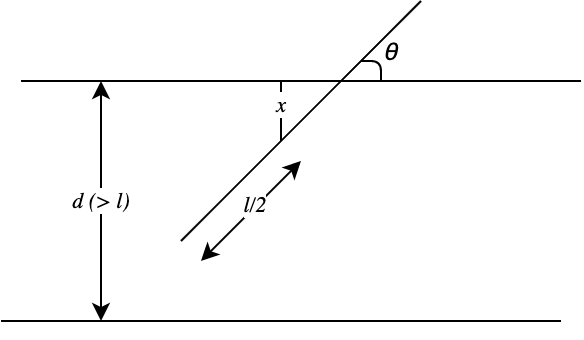
\includegraphics[width=.4\textwidth]{images/P_buffon_needle.png}
 \end{figure}
 
The distance of the midpoint from the closest line is $x$. The needle forms an acute angle $\theta$ with the horizontal line.  The needle length corresponding to the intersection is $x/\sin \theta$. The needle will intersect the line if this distance is less than $l/2$.

We model this using random variables $(X,\Theta)$. It can be seen since the throw is random the vertical orientation is uniformly distributed along with the orientation of the needle. This means that both of the \rv are independent. Since all throws are equally likely the joint PDF will be uniformly distributed over all $x \in [0, d/2]$ and $\theta \in [0,\pi/2]$. Thus this gives us the following joint PDF
\[f_{X,\Theta}=\begin{cases} 
    4/(\pi d) & x \in [0, d/2], \theta \in [0, \pi/2] \\
    0 & \text{otherwise}
\end{cases}\]

The needle can only intersect the line when $X \le (l/2)\sin \Theta$. So the probability of intersection is 
\[P(X \le (l/2)\sin \Theta) = \int_{0}^{\pi/2}\int_{0}^{(l/2)\sin \theta} \frac{4}{\pi d} \, dx \, d\theta = \frac{2l}{\pi d}\] \qed
\end{example}

\subsection{Joint CDFs}
If $X, Y$ are two \rv associated with the same experiment then we define the Joint CDF as
\[\boxed {F_{X,Y}(x,y) = P(X\le x, Y\le y)}\]

The advantage of working with Joint CDFs is that it allows us to deal with both --- discrete and continuous random variable in one shot.

The PDFs can be recovered from CDF by differentiating
\[\boxed{f_{X,Y}(x,y)=\frac{\partial^2{F_{X,Y}}}{\partial x \, \partial y}(x,y)}\]

\subsection{Expectation}
For two jointly continuous \rv $X, Y$ and $Z=g(X,Y)$ is also a \rv for some function $g$. The expected value is given by
\[\E[g(X,Y)]=\int_{-\infty}^{+\infty}\int_{-\infty}^{+\infty}g(x,y)f_{X,Y}(x,y) \, dx \, dy\]

For any scalars $a, b, c$ we have,
\[\E[aX+bY+c]=a\E[X]+b\E[Y]+c\]

\section{Conditioning}
The formulas for conditional probabilities are similar to that of the discrete case except the subtlety that arises because of the event $\{Y=y\}$ which has zero probability.

\subsection{Conditioning a \RV on an event}
The conditional PDF of a continuous \rv given an event $A$ with $P(A)>0$ is defined as a nonnegative function $f_{X|A}(x)$ that satisfies
\[\boxed{P(X \in B| A) = \int_{B}f_{X|A}(x) dx}\]
for any subset $B$ of the real line. For setting $B$ to be entire real line, we obtain the normalization property
\[\int_{-\infty}^{+\infty}f_{X|A}(x) \, dx =1\]
Thus $f_{X|A}$ is a legitimate PDF.

As a special case
\[f_{X|X\in A}(x) = \begin{cases}
   \dfrac{f_X(x)}{P(X\in A)}, & x \in A \\
    0, & \text{otherwise}
\end{cases}\]
Similarly there is a notion of joint conditional PDF of two jointly associated \rv $X,Y$ with joint PDF $F_{X,Y}(x,y)$. For a conditioning event $C=\{(X,Y)\in A\}$, we have
\[f_{X,Y|C}(x,y)=\begin{cases}
    \dfrac{f_{X,Y}(x, y)}{P(C)}, & x \in A \\
     0, & \text{otherwise}
 \end{cases}\]
The conditioning PDF of $X$ can be obtained from the formula
\[f_{X|C}(x) = \int_{-\infty}^{+\infty} f_{X,Y|C}(x,y) dy\]

Finally, there is a version of total probability theorem which involves conditional PDFs: if events $A_1, \ldots, A_n$ form a partition of the sample space then
\[\boxed {f_X(x) = \sum_{i=1}^{n} P(A_i)f_{X|A_i}(x)}\]

\subsection{Conditioning one \RV on Another}
Let $X, Y$ be continuous \rv with joint PDF $f_{X,Y}(x,y)$. For any $y$ with $f_Y(y)>0$, the conditional PDF of $X$ given that $Y=y$, is defined by 
\[\boxed{f_{X|Y}(x|y) = \frac{f_{X,Y}(x,y)}{f_Y(y)}}\]

It is best to think $y$ as a fixed number so that the conditional PDF $f_{X|Y}(x|y)$ is a function of a single variable $x$ with same shape as the $f_{X,Y}(x,y)$ because the denominator doesn't depend on $x$.

Since the following normalization property holds, $f_{X|Y}(x,y)$ is a legitimate PDF for a fixed $y$.
\[\int_{-\infty}^{+\infty}f_{X|Y}(x|y)\,dx=1\]

\subsubsection{Interpretation of conditional PDFs}
Consider two small positive numbers $\delta_1, \delta_2$ and the conditioning event $B={Y\in [y, y+\delta_2]}$, we have
\begin{align*}
    P(X \in [x, x+\delta_1]|Y \in [y, y+\delta_2]) & =\frac{P(X \in [x, x+\delta_1],Y \in [y, y+\delta_2])}{P(Y \in [y, y+\delta_2])} \\
    & \approx \frac{f_{X,Y}(x,y)\delta_1\delta_2}{f_Y(y)\delta_2} \\
    &= f_{X|Y}(x|y)\delta_1
\end{align*}

In other words, $f_{X|Y}(x|y)\delta_1$ provides us with the probability $X \in [x,x+\delta_1]$ given that $Y\in [y, y+\delta_2]$. Since the probability does not depend on $\delta_2$ we can consider the limiting case where $\delta_2 \to 0$ and write
\[P(X\in[x,x+\delta_1]|Y=y) \approx f_{X|Y}(x|y)\delta_1\]
or more generally
\[P(X \in A|Y=y) = \int_{A}f_{X|Y}(x|y) \, dx\]

Note that the event $\{Y=y\}$ is a zero probability event and in discrete case it was left undefined unlike the current formula which is natural.

As in the discrete case, the conditional probability $f_{X|Y}$ is used along with $f_Y(y)$ to calculate the joint PDFs. This approach can be used for modelling the joint probability where the event of $Y$ is specified and then the conditional probability $f_{X|Y}(x|y)$ of $X$ are specified.

\begin{align*}
    f_{X,Y}(x,y) &= f_Y(y)f_{X|Y}(x|y) \\
    f_X(x) &= \int_{-\infty}^{+\infty}f_Y(y)f_{X|Y}(x|y) \, dy
\end{align*}

The above results can be easily extended to more than one variable.

\subsection{Conditional Expectation}
Let $X, Y$ be jointly continuous \rv and let $A$ be an event with $P(A)>0$
\begin{enumerate}
    \item The conditional expectation of $X$ given the event $A$ is defined by 
    \[\E[X|A]=\int_{-\infty}^{+\infty}xf_{X|A}(x) \, dx, \qquad
    \E[X|Y=y] = \int_{-\infty}^{+\infty}xf_{X|Y}(x|y) \, dx\] 
    \item \textbf{The expected value rule}: For a function $g(X)$ we have
    \[\E[g(X)|A] = \int_{-\infty}^{+\infty} g(X) f_{X|A}(x)dx, \qquad 
    \E[g(X)|Y=y] = \int_{-\infty}^{+\infty}g(x)f_{X|Y}(x|y) \, dx\]
    \item \textbf{Total expectation theorem:} Let $A_1,\ldots,A_n$ be disjoint events that form a partition of the sample space and assume that $P(A_i)>0, \; \forall i$. Then,
    \[\E[X] = \sum_{i=1}^{n} P(A_i) \E[X|A_i], \qquad \E[X] = \int_{-\infty}^{+\infty}\E[X|Y=y] f_Y(y) \, dy\]
    \item There are natural analogs for the case of functions of several \rv 
    \[\E[g(X,Y)|Y=y] = \int g(x,y)f_{X|Y}(x|y) dx, \qquad E[g(X,Y)] = \int \E[g(X,Y)|Y=y] f_Y(y) \, dy\]
\end{enumerate}

\section{Independence}
In full analogy to the discrete case we say that the two \rv $X, Y$ are independent if
\[\boxed {f_{X,Y}(x,y) = f_X(x)f_Y(y) \qquad \forall x,y}\]
which is same as
\[f_{X|Y}(x|y) = f_X(x), \quad \forall x,y; \; f_Y(y)>0\]
Some other properties are
\begin{enumerate}
    \item In particular, independence implies
    \[F_{X,Y}(x,y)=P(X\le x, Y\le y)=P(X\le x)P(Y\le y)=F_X(x)F_Y(y)\]
    \item The above can be used to provide a general definition for the independence
    \[F_{X,Y}(x,y) = F_X(x)F_Y(y) \qquad \forall x,y\]
    Even if $X$ is discrete and $Y$ is continuous.
    \item If $X, Y$ are independent then
    \[\E[g(X)h(Y)] = \E[g(X)]\E[h(Y)]\]
    \item The variance of sum of independent random variables is equal to the sum of their variances.
    \begin{center}
        var$(X+Y)$ = var$(X)$ + var$(Y)$
    \end{center}
\end{enumerate}

\section{Continuous Bayes' Rule}
The setting is similar to the discrete case and the only difference is the continuous \rv here. The cases discussed below are based on whether quantity observed or inferred is continuous.

\begin{figure}[h]
    \center
    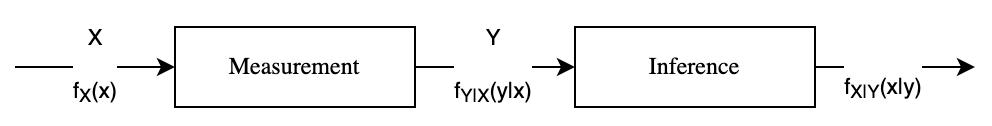
\includegraphics[width=.8\textwidth]{images/P_bayes rule.png}
 \end{figure}

Let the unobserved phenomenon is denoted by a \rv $X$ with known PDF $f_X$. We obtain a measurement $Y$ according to a conditional PDF $f_{Y|X}$. Given the observed value $y$ of $Y$, the inference problem is to evaluate the conditional PDF $f_{X|Y}$.

Note that whatever information is provided by the event $\{Y=y\}$ is captured by the conditional PDF $f_{X|Y}$. It suffices us to calculate this PDF.
\begin{align*}
    f_{X|Y}(x|y) &= \dfrac{f_{X,Y}(x, y)}{f_Y(y)} \\
                &= \dfrac{f_X(x)f_{Y|X}(y|x)}{\int_{-\infty}^{+\infty}f_X(t)f_{Y|X}(y|t) \, dt}
\end{align*}

\subsection{Inference about a discrete \rv}
Let the unobserved phenomenon is described in terms of an event $A$ whose occurrence is unknown. Let $P(A)$ denotes its probability. Let $Y$ be a continuous \rv and assume that $f_{Y|A}$ and $f_{Y|A^c}$ are known. We are interested in $P(A|Y=y)$ of the event $A$, given the that $Y$ takes $y$.

Instead of working with the event zero probability event $\{Y=y\}$, let us work with $\{y \le Y \le y+\delta\}$ where $\delta$ is a small positive number and then take the limit tending to zero. We have using Bayes' rule and assuming $f_Y(y)>0$
\begin{align*}
    P(A|Y=y) & \approx P(A|y \le Y \le y+\delta) \\
             &= \frac{P(A)P(y \le Y \le y+\delta|A)}{P(y \le Y \le y+\delta)} \\
             & \approx \frac{P(A)f_{Y|A}(y)\delta}{f_Y(y)\delta} \\
             &= \frac{P(A)f_{Y|A}(y)}{f_Y(y)}\\
             &= \frac{P(A)f_{Y|A}(y)}{P(A)f_{Y|A}(y)+P(A^c)f_{Y|A^c}(y)}
\end{align*}

The last equality follows because of the total probability theorem.

\subsection{Inference Based on Discrete Observations}
Note that
\begin{align*}
    f_{Y|A}(y) &= \frac{f_Y(y)P(A|Y=y)}{P(A)} \\
               &= \frac{f_Y(y)P(A|Y=y)}{\int_{-\infty}^{+\infty}f_Y(t)P(A|Y=t) \, dt}
\end{align*}

This formula can be used to make an inference about a \rv $Y$ when event $A$ is observed. 
\chapter{Advanced topics on \RV}

Objectives of this chapter are
\begin{enumerate}
    \item deriving the distribution of a function of a \rv(s)
    \item sum of independent \rv and also where the number of \rv is itself random
    \item quantifying the degree of dependence between \rv
\end{enumerate}

\section{Derived Distributions}
Given a continuous \rv $X$ we want to calculate PDF of a \rv $Y=g(X)$ (also called as \textit{derived distribution}). The two step cookbook procedure is as follows:
\begin{enumerate}
    \item Calculate the CDF $F_Y(y)$ using:
    \[F_Y(y)=P(g(X)\le y)=\int_{\{x|g(X)\le y\}}f_X(x) dx\]
    \item Differentiate to obtain the PDF of Y:
    \[f_Y(y)=\frac{d \, F_Y}{dy}(y)\]
\end{enumerate}
More concisely it can be written as:
\begin{center}
    PDF of X $\to$ CDF of X $\to$ CDF of Y $\to$ PDF of Y
\end{center}

\subsection{PDF of a Linear Function of a \RV}
Let $X$ be a continuous \rv with PDF $f_X$ and let $Y=aX+b$ where $a \neq 0$ and $b$ are scalars. Then
\[\boxed{f_Y(y)=\frac{1}{|a|}f_X\left( \frac{y-b}{a}\right)}\]

\begin{remark}
    This equation can be used in proving that the linear function of a Normal \RV is also Normal.
\end{remark}

\subsection{Monotonic Functions}
Suppose that $g$ is strictly monotonic with inverse $h$. Assume that $h$ is differentiable, then the PDF of $Y =g(X)$ in the region where $f_Y(y)>0$ is given by
\[\boxed{f_Y(y)=f_X(h(y)) \left| \frac{dh}{dy}(y) \right|}\]

\subsubsection{Proof}
Suppose that $g$ is monotonically increasing
\[F_Y(y)=P(g(X)\le y)=P(X\le h(y))=F_X(h(y))\]
Differentiating to obtain PDF of Y using chain rule we get
\[f_Y(y)=\frac{dF_Y}{dy}(y)=f_X(h(y))\frac{dh}{dy}(y)\]
Because $g$ is monotonically increasing so will be $h$ so its derivative is non-negative. So the rule follows.

For monotonically decreasing case, we get
\[F_Y(y)=P(g(X)\le y)=P(X \ge h(y))=1-F_X(h(y))\]
and use the chain rule to obtain the above relation.
\qed

\subsubsection{Intuition}

\begin{figure}[h]
    \center
    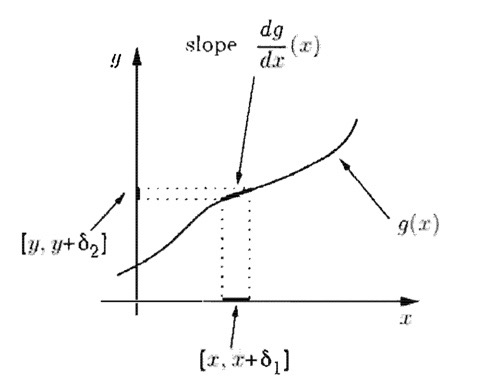
\includegraphics[width=.5\textwidth]{images/P_4_derived_distribution.jpeg}
 \end{figure}

 Consider a small interval $[x,x+\delta_1], \delta_1 \approx 0$ and a monotonically increasing function $g$. The image of this interval is the interval $[y, y+\delta_2]$. We have following based on the slope
 \[\frac{\delta_2}{\delta_1} \approx \frac{dg}{dx}(x)\]
 or in terms of inverse function
 \[\frac{\delta_1}{\delta_2}\approx \frac{dh}{dy}(y)\]

 Note that the event $\{x \le X \le x+\delta_1\}$ is same as the event $\{y\le Y \le y+\delta_2\}$. Thus,
 \begin{align*}
     f_Y(y)\delta_2 & \approx P(y\le Y \le y+\delta_2) \\
          &= P(x \le X \le x+\delta_1) \\
          &= f_X(x)\delta_1
 \end{align*}

This leads to following two relations
 \[f_X(x)=f_Y(y) \cdot \frac{\delta_2}{\delta_1}=f_Y(y)\frac{dg}{dx}(x), \qquad f_Y(y)=f_X(h(y))\cdot \frac{\delta_1}{\delta_2}=\frac{dh}{dy}(y)\]

 \subsection{Function of Two \RV}
 The same cookbook procedure of first finding the CDF and then differentiating it to get PDF also applies when there are multiple \rv

\subsubsection{Example: Romeo \& Juliet}
Romeo and Juliet have a date at a given time and they are late by amount of time (independently of each other) that is exponentially distributed with parameter $\lambda$. What is the PDF of their differences in time of arrival?


Let us denote by $X$ and $Y$ the amount of time by which Romeo and Juliet are late respectively. We want to calculate PDF of $Z=X-Y$. We'll calculate CDF $F_Z(z)$ by considering the cases $z\ge 0$ and $z<0$.
For $z\ge 0$, we have,
\begin{align*}
    F_Z(z) &= P(X-Y \le z) \\
           &= 1 - P(X-Y>z) \\
           &= 1 - \int_{z}^{\infty} \lambda e^{-\lambda x} \left(\int_{0}^{x-z} \lambda e^{-\lambda y} dy \right) dx \\
           &= 1 - \frac{1}{2} e^{-\lambda z}
\end{align*}
For the case $z<0$, we can have a similar calculation but we'll argue in terms of symmetry of the situation. The variables $Z=X-Y$ and $-Z=Y-X$ have the same distribution. We have
\[F_Z(z) = P(Z \le z) = P(-Z\ge -z) = P(Z\ge -z)= 1 - F_Z(-z)=\frac{1}{2} e^{\lambda z}\]

Thus after differentiating the CDF we get the PDF as 
\[f_Z(z) = \frac{\lambda}{2}e^{-\lambda |z|}\]
This is also called as two-sided exponential PDF or Laplace PDF.
\qed

\subsection{Sums of many Independent \RV (Convolution)}
Let $Z=X+Y$ where $X,Y$ be two independent discrete \rv with PMFs $p_X$ and $p_Y$ respectively. Then for any integer $z$,
\begin{align*}
    p_Z(z) &= P(X+Y=z) \\
           &= \sum_{\{(x,y)|x+y=z \}} P(X=x, Y=y) \\
           &= \sum_xP(X=x, Y=z-x) \\
           &= \sum_x p_X(x)p_Y(z-x)
\end{align*}

The resulting PMF $p_Z$ is called as the convolution of PMFs of $X$ and $Y$.

Suppose now that $X$ and $Y$ are independent continuous \rv and we want to find the PDF of $Z=X+Y$.

Note that
\[P(Z\le z|X=x) = P(X+Y\le z|X=x) = P(Y\le z-x)\]

The last equality follows because of independence of $X$ and $Y$.We differentiate both sides w.r.t. $z$ and find that $f_{Z|x}(z|x)=f_Y(z-x)$. Using multiplication rule we get

\[f_{X,Z}(x,z)=f_X(x)f_{Z|X}(z|x)=f_X(x)f_Y(z-x)\]

Finally we obtain
\[f_Z(z)=\int_{-\infty}^{\infty}f_{X,Z}(x,z) dx = \int_{-\infty}^{\infty}f_X(x)f_Y(z-x) dx\]

\subsubsection{Intuition}
\begin{figure}[h]
    \center
    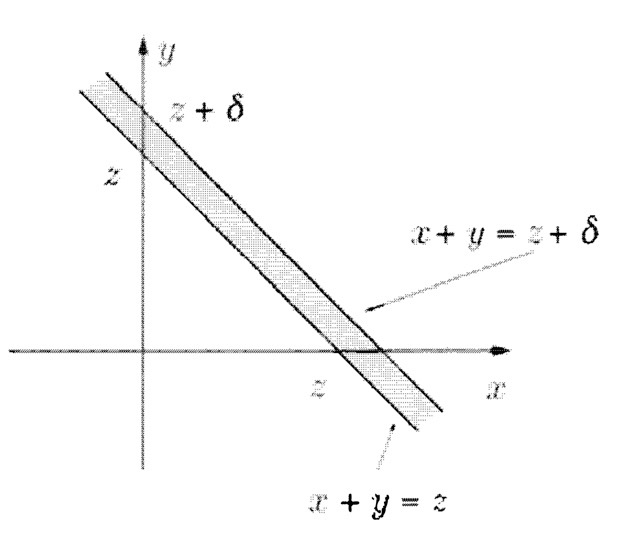
\includegraphics[width=.4\textwidth]{images/P_4_convolution.jpeg}
 \end{figure}

 Consider the strip as shown in the figure with small $\delta$.The probability of the strip is $P(z \le X+Y \le z+\delta) \approx f_Z(z) \delta$
 \begin{align*}
    f_Z(z) \delta &= P(z \le X+Y \le z+\delta) \\
    &= \int_{-\infty}^{\infty}\int_{z-x}^{z-x+\delta} f_X(x)f_Y(y) \, dy \, dx \\
    & \approx \int_{-\infty}^{\infty}f_X(x)f_Y(z-x) \delta \, dx
 \end{align*}
 Canceling $\delta$ on both sides gives the desired result. \qed
 \newline
 \begin{remark}
    Sum or of two normal \rv is normal and scalar multiple of a normal \rv is also normal, therefore for normal \rv $X, Y$ the \rv $aX+bY$ is also normal. 
 \end{remark}

 \subsubsection{Example: Romeo \& Juliet (Difference of \RV)}
 Here's a different solution using convolution.

 Note that the difference of \rv $X-Y$ can be viewed as $X+(-Y)$. We observe that $f_{-Y}(y)=f_Y(-y)$.
 \begin{align*}
     f_{X-Y}(z) &= \int_{-\infty}^{\infty}f_X(x)f_{-Y}(z-x) \, dx \\
      &= \int_{-\infty}^{\infty}f_X(x)f_Y(x-z) \, dx \\
      &= \int_{z}^{\infty} \lambda e^{-\lambda x} \lambda e^{-\lambda(x-z)} \, dx\\
      &= \lambda^2 e^{\lambda z} \int_{z}^{\infty} e^{-2 \lambda x} \, dx \\
      &= \frac{\lambda}{2} e^{-\lambda z}
 \end{align*}
 The answer for the case $z<0$ is obtained using symmetry, since $X, Y$ are identically distributed,
 \[f_{X-Y}(z)=f_{Y-X}(z)=f_{-(X-Y)}(z)=f_{X-Y}(-z)\] \qed

 \subsection{Graphical Calculation of Convolution}

 Let $t$ be a dummy variable and suppose that we have two PDFs $f_X(t)$ and $f_Y(t)$. The graphical evaluation consists of the following steps:
 \begin{enumerate}
     \item We plot $f_Y(z-t)$ as a function of $t$. The plot has the same shape as that of $f_Y(t)$ but first flipped and then shifted to left/right depending whether $z<0$ or $z>0$.
     \item We place the plots of $f_X(t)$ and $f_Y(z-t)$ on top of each other and form their product.
     \item We calculate $f_Z(z)$ by calculating the integral of the product of the plots.
 \end{enumerate}

 By varying the amount of shifting as controlled by $z$ we can calculate for any $z$.

 \section{Covariance and Correlation}
 The covariance of two \rv $X, Y$ is denoted by cov$(X,Y)$ and is defined as
 \[\boxed{\text{cov}(X,Y)=\E\big[(X-\E[X])(Y-\E[Y])\big]}\]
 A zero covariance means that the \rv are uncorrelated. A positive covariance means that the values of $X-\E[X]$ and $Y-\E[Y]$ obtained in a single experiment "tend" to have same sign.

 \begin{remark}
    If $X, Y$ are independent then the covariance is zero but the converse may not be true.
 \end{remark}

 An alternative formula is 
 \[\boxed{\text{cov}(X,Y)=\E[XY]-\E[X]\E[Y]}\]

 Simple properties of covariances are
 \begin{align*}
     \text{cov}(X,X) &= \text{var}(X) \\
     \text{cov}(X, aY+b) &= a \cdot \text{cov}(X, Y) \\
     \text{cov}(X, Y+Z) &=\text{cov}(X,Y)+\text{cov}(X,Z)
 \end{align*}

 The \textbf{correlation coefficient} $\rho(X,Y) \in [-1, 1]$ is defined as 
 \[\boxed {\rho(X,Y) =\frac{\text{cov}(X,Y)}{\sqrt{\text{var}(X) \text{var}(Y)}} }\]

 \subsection{Variance of Sum of \RV}
 The covariance can be used to calculate the variance of sum of several \rv (not necessarily independent). In particular if $X_1, \ldots, X_n$ are \rv with finite variances, then
 \[\text{var}(X_1+X_2)=\text{var}(X_1)+\text{var}(X_2)+2\text{cov}(X_1, X_2)\]
 or more generally
 \[\text{var}\left(\sum_{i=1}^{n}X_i\right)=\sum_{i=1}^n\text{var}(X_i) + \sum_{i \neq j}\text{cov}(X_i, X_j)\]

 \section{Iterated Expectations}
 We revisit the conditional expectation of a \rv $X$ given another \rv $Y$ and we treat it as a \rv whose value is determined by $Y$.

 We define $\E[X|Y]$ to be a \rv that takes the value $\E[X|Y=y]$ when $Y$ takes a value $y$. Since $\E[X|Y=y]$ is a function of $y$, $\E[X|Y]$ is a \textit{function} of $Y$.

 Since $\E[X|Y]$ is a \rv it has expectation of its own,
 \[ \E[\E[X|Y]] = \E[X] = \begin{cases}
    \displaystyle\sum_y p_Y(y) \E[X|Y=y], & Y \text{ discrete} \\
    \displaystyle\int_{-\infty}^\infty f_Y(y)\E[X|Y=y] \, dy, & Y \text{ continuous}
 \end{cases} \]

 The equality is also called as 
 \[\boxed{ \textbf{Law of Iterated Expectations:} \quad \E[\E[X|Y]]=\E[X] }\]

 This law is the abstract notation of the total expectation theorem which loosely says that the average in whole is the weighted average of the parts where weights are the probabilities.
 
 For a function $g$, the following property holds (because $g(Y)$ will be a constant)
 \[\E[Xg(Y)|Y]=g(Y)\E[X|Y]\]

 \subsection{Conditional Expectation as an Estimator}
 If $Y$ provides information about $X$ then $\hat X = \E[X|Y]$ is an estimator for $X$ given $Y$. The estimation error is $\tilde X = \hat X - X$ that satisfies
 \[\E[\tilde X | Y]=\E[\hat X - X |Y]=\E[\hat X|Y]-\E[X|Y]=\hat X - \hat X = 0\]

 Thus the \rv $\E[\tilde X |Y]$ is identically zero. By using law of iterated expectations $\E[\tilde X]=\E[\E[\tilde X|Y]]=0$. This reassures that the estimation error doesn't have any systematic upward or downward bias.

 We now show that $\tilde X$ is uncorrelated with $\hat X$. Using law of iterated expectations
 \[\E[\tilde X \hat X]=\E[\E[\tilde X \hat X|Y]]=\E[\hat X \E[\tilde X|Y]]=0\]
 where the last two equality follows because $\hat X$ is completely determined by $Y$. It follows that 
 \[\text{cov}(\tilde X,\hat X)=\E[\tilde X \hat X]-\E[\tilde X]\E[\hat X] = 0 - \E[\hat X] \cdot 0=0\]
 Thus $\hat X$ and $\tilde X$ are uncorrelated.

 \subsection{Conditional Variance}
 We introduce the \rv 
 \[\text{var}(X|Y)=\E \big [(X-\E[X|Y])^2 \, | \,Y \big ]=\E[\tilde X ^2 | Y]\]
 using the fact that $\E[\tilde X]=0$ and the law of iterated expectations, the variance of the estimation error is
 \[\var(\tilde X)=\E[\tilde X ^2]=\E[\E[\tilde X ^2|Y]]=\E[\var(X|Y)]\]

 Therefore $\var(X)=\var(\tilde X) + \var(\hat X)$ which gives us
 \[\boxed{ \textbf{Law of Total Variance:} \quad \var(X)=\E[\var(X|Y)]+\var(\E[X|Y])}\]

 \subsubsection{Intuitive Example}
 Suppose that we want to find the total variance of quiz scores of a class. Suppose that $X$ is the quiz score of the student and $Y\in \{1,\ldots,k\}$ denotes the section of the student.
 
 Let $n_s$ be the number of students in section $s$ and $n$ be the total number of students. We interpret the total variance formula as:
 \begin{enumerate}
     \item $\E[\var(X|Y)]$ is the variability within the sections and is the weighted average of section variances where the weight is proportional to its size.

     $\var(X|Y=s)$ is the variance of quiz scores \textit{within} section $s$. Thus
     \[\E[\var(X|Y)]=\sum_{s=1}^{k}P(Y=s)\var(X|Y=s)=\sum_{s=1}^{k}\frac{n_s}{n}\var(X|Y=s)\]
     \item $\var(\E[X|Y])$ is the variability of the average scores ($\E[X|Y]$) \textit{between} the sections.
 \end{enumerate}

 Combining the values we get $\var(X)=\var(\E[X|Y])+\E[\var(X|Y)]$

 \section{Transform}

 \section{Sum of random number of independent random variables}

 We consider the sum
 \[Y=X_1+\cdots+X_N\]
 where $N$ is a \rv that takes non negative values and $X_i$'s are identically distributed random variables. We assume $N,X_1,\ldots$ are independent so that any finite subset of \rv are also independent. Let $E[X]$ and $\var(X)$ denote the common mean and variance, respectively, of the $X_i$.

 Fix a nonnegative integer $N=n$. Since the sum $X_1+\cdots+X_n$ is independent of $N$ and therefore is independent of $\{N=n\}$.
 \begin{align*}
    \E[Y|N=n] &= \E[X_1+\cdots+X_N|N=n] \\
    &= \E[X_1+\cdots+X_n|N=n] \\
    &= \E[X_1+\cdots+X_n] \\
    &= n\E[X]
 \end{align*}

 Since it is true for every nonnegative integer $n$, so $\E[Y|N]=N\E[X]$. Using law of iterated expectations we get
 \[\E[Y]=\E[\E[Y|N]]=\E[N\E[X]]=\E[N]\E[X]\]
 Similarly,
 \begin{align*}
    \var(Y|N=n) &= \var(X_1+\ldots+X_N|N=n) \\
    &= \var(X_1+\ldots+X_n|N=n) \\
    &= n \, \var(X)
 \end{align*}
 Since this is true for every $N$ we get $\var(Y|N)=N\var(X)$
 We now use law of total variance to obtain
 \begin{align*}
     \var(Y) &= \E[\var(Y|N)] + \var(\E[Y|N]) \\
     &= \E[N\var(X)] + \var(N\E[X]) \\
     &= \var(X)\E[N] + (\E[X])^2\var(N)
 \end{align*}

 \textbf{See the transform method on p. 241 and its examples}
\chapter{Bernoulli and Poisson Processes}
A stochastic process is a mathematical model of a probabilistic experiment that evolves in time and generates a sequence of numerical values. For example, the sequence of daily prices of a stock.

Each numerical value in the sequence is modeled by a random variable, so a stochastic process  is simply a  (finite or  infinite) sequence of random variables. We are still dealing with a single basic experiment that involves outcomes governed by a probability law, and random variables that inherit their probabilistic properties from that law.

However, stochastic processes involve some change in emphasis over our earlier models, such as:
\begin{enumerate}
    \item We tend to focus on the \textit{dependencies} in the sequence of values generated by  the process. For example, how do  future  prices of a stock depend on past values?
    \item We  are often interested in \textit{long-term averages} involving the entire sequence of generated values. For example, what is the fraction of time that a machine is idle?
    \item We  sometimes wish to characterize the \textit{likelihood} or frequency of certain boundary events. What is the frequency with which some buffer in a computer net­work overflows with data?
\end{enumerate}
There is a wide variety of stochastic processes, but in this book we will only discuss two major categories
\begin{enumerate}
    \item [Arrival] The processes in which occurrences have a characteristic of "arrival". We  will focus on models in which the interarrival times (the times between successive arrivals) are independent \rv. We consider discrete time arrivals and interarrivals (Bernoulli processes) and continuous arrivals and exponentially distributed interarrivals (Poisson process).
    \item [Markov] Experiments that evolve in time and in which the future evolution exhibits a probabilistic dependence on the past. However, we assume a very special type of dependence: the next value depends on past values only through the current value.
\end{enumerate}

\section{Bernoulli Process}
Bernoulli Process can be visualized as a sequence of independent coin tosses where each toss has a fixed probability $p$ which is independent of other trails.

Formally, Bernoulli process is a sequence of \textbf{independent} Bernoulli \RV $X_1,X_2,\ldots$ with
\[
    \Pr(X_i) = \begin{cases}
        \Pr(\text{success at the ith trial)} &= p \\
        \Pr(\text{failure at the ith trial)} &= 1-p
    \end{cases}
\]

Some \rv associated with the Bernoulli Process and their properties
\begin{enumerate}
    \item The binomial with parameters $p$ and $n$. This is the number $S$ of successes in $n$ independent trials. Its PMF, mean, and variance are
    \begin{align*}
        p_S(k) &= \binom{n}{k}p^k(1-p)^{n-k}, \quad k = 0,1,\ldots,n \\
        \E[S] &= np \\
        \var(S)&=np(1-p)
    \end{align*}
    \item The geometric with parameter $p$. This is the number $T$ of trials up to (and including) the first success. Its PMF, mean, and variance are
    \begin{align*}
        p_T(t) &= (1-p)^{t-1}p, \quad t=1,2,\ldots\\
        \E[T]&=1/p\\
        \var(T)&=\frac{1-p}{p^2}
    \end{align*}
\end{enumerate}

\subsection{Independence and Memorylessness}
The independence assumption underlying the Bernoulli process has important implications, including a memorylessness property.
\begin{definition}[Memorylessness]
    Whatever has happened in past trials provides no information on the outcomes of future trials.
\end{definition}

We develop some intuition as this property leads to quick and simple solutions to difficult problems. 
\begin{itemize}
    \item [independence] Let us start by considering random variables that are defined in terms of what happened in a certain set of trials. Consider two \rv $Y=(X_1+X_3)X_6X_7$ and $Z=X_2(X_4+X_5)$ are independent because of no common element. This is generalization of fact that functions of independent \rv are independent.
    \item [fresh start] Suppose now that the Bernoulli process has been running for $n$ time steps with observed values as $X_1,\ldots,X_n$. The sequence of future trials $X_{n+1},X_{n+2},\ldots$ are independent Bernoulli trials and therefore a Bernoulli process. Starting from any given point in time, the future is also modeled by a Bernoulli process, which is independent of the past.
    \item [first success] The time until first success is a geometric \rv and so failing first $n$ trials provides us with no information about the probability of first success. Due to fresh-start the \rv for the first success after $n$ trials remains unchanged.
    \[
        \Pr(T-n=t|T>n)=(1-p)^{t-1}p=\Pr(T=t), \quad t=1,2,\ldots
    \]
\end{itemize}

\subsection{Interarrival times}
Consider $T_i$ to to be the interarrival time between the $i-1^{th}$ and $i^{th}$ arrival. Since Bernoulli processes have a fresh-start property, $T_i$'s are independent of each other as the time beginning after the $(i-1)^{th}$ arrival tells us nothing about the future. This gives us an alternate definition of the Bernoulli process.

\begin{definition}[Bernoulli Process]
    Start with a sequence of geometric independent \rv $T_1, T_2,\ldots$ with same parameter $p$ and let these be interarrival times. Record a success at time $T_1, T_1+T_2, T_1+T_2+T_3, \ldots$
\end{definition}

\begin{example}
    It has been observed that after a rainy day. the  number of days until it rains again is geometrically distributed with parameter $p$. independent of the past. Find the probability that it rains on both the 5th and the 8th day of the month.

    If we consider the independence of the trails then the answer is $p^2$. \qed
\end{example}

\subsection{$k^{th}$ Arrival time}

The time of the $k^{th}$ arrival $Y_k=T_1+\cdots+T_k$, where $T_i$'s are geometric \rv has
\begin{align}
    \E[Y_k]&=\E[T_1]+\cdots+\E[T_k]=k/p\\
    \var(Y_k)&=\var(T_1)+\cdots+\var(T_k)=\frac{k(1-p)}{p^2}\\
    \label{pascal_pmf}
    p_{Y_k}&=\binom{t-1}{k-1}p^k(1-p)^{t-k}, \quad t=k,k+1,\ldots,
\end{align}
where \ref{pascal_pmf} is known as Pascal PMF of order $k$.

\subsection{Splitting and merging of Bernoulli process}
Consider a Bernoulli process of arrivals with probability of each arrival as $p$ independent of other arrivals. Suppose that with probability $q$ we either keep it or with probability $1-q$ we discard it. The probability of keeping the arrival is now $pq$ and this it is also a Bernoulli process with probability $pq$. Similarly the discarded arrivals also constitute a Bernoulli process with probability $p(1-q)$.

\begin{remark}
    To prove that a process is Bernoulli we need that the probability of each arrival must be same for every arrival and is independent from other arrivals. The arrivals were independent before splitting and thus remains independent after splitting.
\end{remark}

Similarly in case of merging, if the probabilities of the processes are $p$ and $q$ respectively, then the merged process will be a Bernoulli process with probability $(1-p)(1-q)$ or $p+q-pq$.

\subsection{The Poisson approximation to the Binomial}
The number of successes in $n$ independent Bernoulli trails is a Bernoulli \rv with parameters $n$ and $p$ with mean as $np$. If we let $n$ grow large and simultaneously decrease $p$ to keep the mean constant, we can approximate Poisson process as Bernoulli process with large trails and small probability of each success.

\begin{enumerate}
    \item The poisson \rv $Z$ with parameter $\lambda$ takes nonnegative integer values described by the PMF 
    \[p_Z(k)=e^{-\lambda}\frac{\lambda^k}{k!}, \quad k=0,1,\ldots,\]
    The mean and variance are $\E[Z]=\var(Z)=\lambda$.
    \item The binomial probability \[p_S(k)=\binom{n}{k}p^k(1-p)^{n-k}\] converges to $p_Z(k)$ as $n \to \infty$ and $p=\lambda/n$, while keeping $\lambda$ constant.
\end{enumerate}

\section{Poisson process}
The Poisson process is a continuous-time analog of the Bernoulli process and applies to situations where there is no natural way of dividing time into discrete periods.

\begin{example}[Traffic Accidents]
    Suppose that to model traffic accidents we keep a 1-minute interval and mark a "success" if any accidents happen in that interval. This can be a bernoulli process as the time slots are independent with same probability.
    
    It is possible to have two or more accidents happening at the same time but Bernoulli process does not track the exact number of accidents. To get around this, we can choose a smaller time interval but what would it be? a second? a millisecond? Instead, we use the limiting case and arrive at continuous time model. \qed
\end{example}

For an arrival process that evolves in continuous-time, we define
\[P(k,\tau)=P(\text{exactly } k \text{ arrivals happen during interval of length } \tau)\]

We also assume that the probability is same for all intervals of same length $\tau$. We also introduce an arrival rate or intensity of the process as $\lambda$.

\begin{definition}[Poisson process]
    An arrival process is called a Poisson Process with rate $\lambda$ if it satisfies
    \begin{enumerate}
        \item [time-homogeneity] $P(k,\tau)$ of $k$ arrivals is the same for all intervals of length $\tau$.
        
        \textit{All arrivals are equally likely at all times. Analogous to Bernoulli Bernoulli processes having same success probability of each interval as $p$.}

        \item [independence] The number of arrivals during a period is independent of the history of arrivals outside this interval.

        \textit{Analogous to Bernoulli trails being independent of each other.}

        \item [small-interval] The probabilities $P(k,\tau)$ satisfy
        \begin{align*}
            P(0,\tau) &= 1-\lambda\tau+o(\tau)\\
            P(1,\tau) &= \lambda\tau+o_1(\tau)\\
            P(k,\tau) &= o_k(\tau), \quad k=2,3,\ldots
        \end{align*}
        where $o(\tau)$ and $o_k(\tau)$ are asymptotic notations satisfying $\lim_{\tau \to 0}\frac{o_k(\tau)}{\tau}=0$.

        \textit{There can be atmost one arrival with probability $\lambda\tau$ in a small interval $\tau$.}
    \end{enumerate}
\end{definition}

\subsection{Number of Arrivals in an Interval}
Consider a time interval of length $\tau$ and partition it into $\tau/\delta$ periods of small length $\delta$. The probability of two occurrence can be neglected (by \textit{small-interval} property). Different slots are independent (by \textit{independence} property).

Therefore, the probability $P(k, \tau)$ is same as binomial probability of $k$ success in $n=\tau/\delta$ Bernoulli trials with $p=\lambda\delta$.

If $\delta \to 0$, then according to previous section, binomial PMF converges to Poisson PMF with parameter $\lambda\tau$.

\[\boxed{P(k, \tau)=e^{-\lambda\tau}\frac{(\lambda\tau)^k}{k!}, \quad k=0,1,\ldots}\]

\begin{remark}
    The small interval property can be proved by taylor series expansion of above formula.
\end{remark}

The probability law for the first arrival is
\[F_T(t)=\Pr(T\le t)=1-\Pr(T>t)=1-P(0,t)=1-e^{-\lambda t}, \quad t\ge 0\]
Differentiating the CDF $F_T(t)$, we obtain
\[\boxed{f_T(t)=\lambda e^{-\lambda t}, \quad t\ge 0}\]

\subsection{Independence and Memorylessness}
The Poisson process has properties such as
\begin{itemize}
    \item independence of non-overlapping time sets --- For any given time $t>0$, the history of the process after time $t$ is also a Poisson process, and is independent from the history of the process until time $t$.
    \[\Pr(\bar T-t>s)=\Pr(0 \text{ arrivals during }[t,t+s])=P(0,s)=e^{-\lambda s}\]
    \item memorylessness of interarrival time distribution --- Let $t$ be a given time and let $\bar T$ be the time of first arrival after $t$. Then $\bar T -t$ has an exponential distribution with parameter $\lambda$ and is independent of ths history of the process until time $t$.
\end{itemize}
Because Poisson process can be viewed as a limiting case of Bernoulli, therefore it inherits the properties.

\begin{example}[Independence]
    You go to a bank and see all three tellers are busy serving customers and its your turn next. Assuming each customer's service time is identically distributed exponential \rv, what is the probability that you'll be the last one to leave?

    1/3. The time when you'll start serviced, the PDF of the other customers is same as yours because of memorylessness.
\end{example}

\begin{definition}[Poisson Process (Alternative)]
    Start with a sequence of independent \rv $T_1, T_2,\ldots,$ with common parameter $\lambda$ and let these be interarrival times. Record an arrival at $T_1, T_1+T_2, T_1+T_2+T_3,\ldots$, etc.
\end{definition}

\subsection{The $k$th Arrival Time}
The time $Y_k$ of $k$th arrival is equal to $T_1+T_2+\cdots+T_k$ of $k$ independent identically distributed \rv with 
\begin{itemize}
    \item mean and variance as
    \[\E[Y_k]=\E[T_1]+\cdots+\E[T_k]= k/\lambda\]
    \[ \var(Y_k)=\var(T_1)+\cdots+\var(T_k)=k/\lambda^2\]
    \item The PDF of $Y_k$ is given by
    \[f_{Y_k}(y)=\frac{\lambda^ky^{k-1}e^{-\lambda y}}{(k-1)!}, \quad y\ge 0\]
    and is known is Erlang PDF of order $k$.
\end{itemize}

\begin{remark}
    For a small $\delta$, $\delta f_{Y_k}(y)$ gives the probability of $k^{th}$ arrival in the interval $[y,y+\delta]$, i.e. $y\le Y_k \le y+\delta$.
\end{remark}

\subsection{Splitting and Merging of Poisson Process}
Similar to Bernoulli process, 
\begin{enumerate}
    \item [split] An arrival in Poisson process can be kept with probability $p$ and this the splitting is a Poisson process with arrival rate $\lambda p$.
    \item [merge] Two Poisson process with arrival rates as $\lambda_1$ and $\lambda_2$ when merged results in a Poisson Process with rate $\lambda_1 + \lambda_2$. An arrival in merged process has probability $\lambda_1/(\lambda_1+\lambda_2)$ of originating from the first process.
\end{enumerate}
\begin{remark}
    Processes obtain by splitting a Poisson process are independent.
\end{remark}

\subsection{Random Incidence Paradox}

\begin{center}
\tikzset{every picture/.style={line width=0.75pt}} %set default line width to 0.75pt
\begin{tikzpicture}[x=0.75pt,y=0.75pt,yscale=-1,xscale=1]
%uncomment if require: \path (0,300); %set diagram left start at 0, and has height of 300

\draw    (119.5,120) -- (479.5,121) ;
\draw    (149.5,90) -- (149.5,130) ;
\draw    (450.5,90) -- (450.5,130) ;
\draw    (305.5,116) -- (296.5,126) ;
\draw    (319.5,100) -- (449.5,100.98) ;
\draw [shift={(451.5,101)}, rotate = 180.43] [color={rgb, 255:red, 0; green, 0; blue, 0 }  ][line width=0.75]    (10.93,-3.29) .. controls (6.95,-1.4) and (3.31,-0.3) .. (0,0) .. controls (3.31,0.3) and (6.95,1.4) .. (10.93,3.29)   ;
\draw    (289.5,101) -- (152.5,101) ;
\draw [shift={(150.5,101)}, rotate = 360] [color={rgb, 255:red, 0; green, 0; blue, 0 }  ][line width=0.75]    (10.93,-3.29) .. controls (6.95,-1.4) and (3.31,-0.3) .. (0,0) .. controls (3.31,0.3) and (6.95,1.4) .. (10.93,3.29)   ;
\draw    (305.5,126) -- (296.5,116) ;

\draw (299,91) node [anchor=north west][inner sep=0.75pt]  [font=\normalsize] [align=left] {L};
\draw (293.5,134) node [anchor=north west][inner sep=0.75pt]   [align=left] {t*};
\draw (144,133) node [anchor=north west][inner sep=0.75pt]   [align=left] {U};
\draw (445,130) node [anchor=north west][inner sep=0.75pt]   [align=left] {V};
\end{tikzpicture}
\end{center}
For a fixed time instant $t^*$, the corresponding interval $[U,V]$ consists of elapsed time $t^* - U$ and remaining time $V-t^*$. These two times are independent and are exponentially distributed with parameter $\lambda$, so the PDF of their sum is Erlang of order two.

This misconception arises an observer is more likely to fall into larger intervals than smaller intervals. Thus the expected length observed is larger than actual expected length.

\begin{example}[Random Incidence on a Non-Poisson Arrival Process]
    Imagine a bus station at which buses arrive with interarrival time alternating between 5 and 55 mins. The average interarrival time is therefore 30 mins. A person shows up at the bus station with all time points in an hour being equally likely.
    The probability of falling in 5 min interval is 1/12 and in 55 min interval is 11/12.
    \[\text{(Expected interarrival time)} \quad 5 \cdot \frac{1}{12} + 55 \cdot \frac{11}{12}=50.83 \gg 30\]
\end{example}

\begin{example}[Questioning a rider from an empty bus]
    Consider the task of calculating percent utilization of buses in a city. There are two approaches
    \begin{enumerate}
        \item Choose a random set of buses and calculate the average riders in it.
        \item Pick random people and ask the number of people that were there in the bus.
    \end{enumerate}
    The second approach is biased upwards because it is more likely for a person to be from a bus with large riders than from nearly empty bus. Empty buses will not be taken into account as there will not be any rider that can account for it.
\end{example}

\section{Sums of \RV}
Let $N,X_1,X_2,\ldots$ be independent \rv and $N$ takes non-negative integer values. Let $Y=X_1+\cdots+X_N$ for positive values of $N$ and $Y=0$ for $N=0$.

\begin{center} \begin{tabu}{|c|c|c|}
    \hline $X_i$ & $N$ & $Y$ \\ \hline
    Bernoulli ($p$) & Binomial ($m, q$) & Binomial ($m, pq$) \\
    Bernoulli ($p$) & Poisson ($\lambda$) & Poisson ($\lambda p$) \\
    Geometric ($p$) & Geometric ($q$) & Geometric ($pq$) \\
    Exponential ($\lambda$) & Geometric ($q$) & Exponential ($\lambda q$)\\
    \hline
\end{tabu} \end{center}

\subsection{Sum of large number of independent arrival process}
The sum of a large number of (not necessarily Poisson) independent arrival processes, can be approximated by a  Poisson process with arrival  rate equal to the sum of the individual arrival  rates. The component processes must have a small rate relative to the total (so that none of them imposes its probabilistic character on the total arrival process) and they must also satisfy some technical mathematical assumptions. Therefore, this property leads to abundance of Poisson-like processes in practice.

For example, the telephone traffic originating in  a city consists of many components, reflecting the phone calls placed by a resident, can be modelled by a Poisson process. Need not be Poisson because some makes calls in batches and usually cannot initiate a second call while on the first call. For the same reasons, auto accidents in a city, customer arrivals at a store, etc tend to be Poisson-like.
\chapter{Markov Chains}
\newcommand*{\MC}{Markov Chains}
Bernoulli and Poisson process are memoryless and future outcomes do not depend on past. In the models we consider here, past has bearing on the future and therefore the model changes state with transition probabilities between states.

\section{Discrete-time Markov Chains}
The state changes at certain discrete time instants, indexed by an integer variable $n$. At each time step $n$, the state is denoted by $X_n$.

\begin{definition}[State space]
    The set of possible states of the model. We assume finite set of states $\mathcal S =\{1,\dots,m\}$.
\end{definition}
\begin{definition}[Transition probabilities $p_{ij}$]
    Whenever state happens to be $i$, there is probability $p_{ij}$ that the next state is equal to $j$.
    \[p_{ij}=\Pr(X_{n+1}=j|X_n=i). \quad i,j \in \mathcal{S}\]
\end{definition}

\subsubsection{Properties of transition probabilities are}
\begin{itemize}
    \item They are independent of the past and how state $i$ is reached.
    \[\Pr(X_{n+1}=j|X_n=i, X_{n-1}, \ldots, X_{0})=\Pr(X_{n+1}=j|X_n=i)=p_{ij}\]
    This is true at all times, for all states and for all sequences of past states.
    \item The transition probabilities are non-negative and sum to one.
    \[\sum_{j=0}^m p_{ij}=1, \quad \forall i\]
\end{itemize}

\begin{remark}
    In some cases where there is a dependence in the previous states, we can encode the dependency by changing the states in a way to eliminate the dependency.
\end{remark}
\subsection{Probability of a path}
Given a \MC we can compute the probability of any sequences of states by using multiplication rule.
\begin{align*}
    \Pr(X_0=i_0,X_1=i_1,\ldots,X_n=i_n) &= \Pr(X_n|X_1=i_1,\ldots,X_{n-1}=i_{n-1})\Pr(X_1=i_1,\ldots,X_{n-1}=i_{n-1}) \\
    &= \Pr(X_n|X_n=i_{n-1})\Pr(X_1=i_1,\ldots,X_{n-1}= i_{n-1}) \\
    &= p_{i_{n-1} n}\Pr(X_1=i_1,\ldots,X_{n-1}=i_{n-1}) \\
    &= p_{i_{n-1}n} \ldots p_{i_0i_1} \Pr(X_0=i_0)
\end{align*}

\subsection{$n$-step Transition Probabilities}
$r_{ij}(n)$ is the probability that the state after $n$ time periods will be $j$, given that the current state is $i$. It can be calculated using the following basic recursion, known as the Chapman-Kolmogorov equation.
\[r_{ij}(n)=\begin{cases}
    \sum_{k=1}^{m}r_{ik}(n-1)p_{kj} & \quad n>1 \\
    p_{ij} & \text{n=1}
\end{cases}\]

\section{Classification of States}
We now classify states based on their long-term frequency with which they are visited.

\begin{definition}[Accessible]
    A state $j$ is accessible from state $i$ iff $r_{ij}(n)$ is positive. In other words, there is a path $i,i_1,\ldots,i_{n-1},j$ which starts at $i$ and ends at $j$, in which the transitions $(i,i_1), (i_1,i_2), \ldots, (i_{n-1},j)$ have positive probability.
\end{definition}
Let $A(i)$ be the set of states accessible from $i$. For a recurrent state $i$, $A(i)$ is called as a recurrent class.
\begin{definition}[Recurrent]
    State $i$ is recurrent if for every state $j\in A(i)$ we have $i \in A(j)$. That is, the set of states which are accessible from each other are called as recurrent.
\end{definition}
\begin{remark}
    A set of recurrent states form a strongly connected component.
\end{remark}
\begin{definition}[Transient]
    A state which is not recurrent.
\end{definition}
A transient state can be visited only a finite number of times because every time you visit that state there is a positive probability of reaching a state from which there is no coming back. This is not the case with recurrent state.

There must exist at least one recurrent class.

\subsection{Periodicity}
A recurrent class is called periodic if it can be decomposed into $d>1$ disjoint subsets $S_1,\ldots,S_d$ so that all transitions from one subset lead to next subset.
\[\text{if } i\in S_k \text{ and } p_{ij}>0, \quad \text{then } \begin{cases}
    S_{k+1} & k=1,\ldots, d-1 \\
    S_1 & k=d
\end{cases}\]

For a periodic recurrent class $R$ at a given positive time $n$ and state $i$ there exists one or more states with $r_{ij}(n)=0$. Thus starting from a state $i$ only a set of states are accessible at a given time. 

This gives us a way to test aperiodicity. If there is a special time $n\ge 1$ and a special state $i\in R$ from which all states in $R$ can be reached then $R$ is aperiodic. Converse is also true if $R$ is aperiodic then there exists a time $n$ such that $r_{ij}(n)>0, \forall i,j \in R$.

\section{Steady-State Behavior}
We're interested in values of $r_{ij}(n)$ when $n$ is very large. If there are more than one recurrent classes then the limiting values of $r_{ij}(n)$ depends on the initial state. So we'll restrict us with a single recurrent class plus some transient states.
\begin{remark}
    The asymptotic behavior of a multiclass chain can be understood in terms of the asymptotic behavior of a single-class chain.
\end{remark}
The conditions required for steady state values are
\begin{enumerate}
    \item Single recurrent class
    \item Aperiodicity
\end{enumerate}
Therefore we can have limiting probabilities $\pi_j$ of ending up in state $j$ independent of initial state after a long time.
\[\pi_j\approx \Pr(X_n=j), \quad \text{when } n \text{ is large}\]

\begin{theorem}[Steady-State convergence]
    Consider a Markov chain with a single recurrent class, which is aperiodic. Then, the states j are associated with steady-state probabilities $\pi_{j}$ that have the following properties.
    \begin{enumerate}
        \item For each $j$, we have 
        \[\lim_{n\to \infty} r_{ij}(n)=\pi_j, \quad \forall i\]
        \item The $\pi_j$ are the unique solution to the balance equations
        \begin{align*}
            \pi_j &= \sum_{k=1}^m \pi_k p{kj}, \quad, j=1,
            \ldots, m\\
            1 &= \sum_{k=1}^m \pi_k
        \end{align*}
        \item We have \[\pi_j \begin{cases}
            =0 & \text{ for all transient states }j \\
            >0 & \text{ for all recurrent states }j
        \end{cases}\]
    \end{enumerate}
\end{theorem}

\subsection{Long-Term Frequency Interpretations}

We can interpret the steady-state probabilities in terms of expected state frequencies.

For a Markov chain with a single class which is aperiodic, the steady-state probabilities $\pi_j$ satisfy
\[\pi_j=\lim_{n\to \infty}\frac{v_{ij}(n)}{n}\]

where $v_{ij}$ is the expected number of visits starting to state $j$ starting from state $i$.

Let $q_{jk}(n)$ be the expected number of transitions that take the state from $j$ to $k$. Then regardless of the initial state
\[\lim_{n \to \infty}\frac{q_{jk}(n)}{n}=\pi_j p_{jk}\]

Using the above interpretations the balance equation make sense intuitively
\[\sum_{k=1}^m\pi_k p_{kj}=pi_j\]
because the expected frequency $\pi_j$ of visits to $j$ is the sum of expected frequencies $\pi_k p_{kj}$ of transitions that lead to $j$.

\begin{figure}[!h]
    \centering
    \begin{center}


    \tikzset{every picture/.style={line width=0.75pt}} %set default line width to 0.75pt        

    \begin{tikzpicture}[x=0.75pt,y=0.75pt,yscale=-1,xscale=1]
    %uncomment if require: \path (0,300); %set diagram left start at 0, and has height of 300
    
    %Shape: Circle [id:dp1080866293664855] 
    \draw   (168.74,89.13) .. controls (168.74,80.22) and (175.96,73) .. (184.87,73) .. controls (193.78,73) and (201,80.22) .. (201,89.13) .. controls (201,98.04) and (193.78,105.26) .. (184.87,105.26) .. controls (175.96,105.26) and (168.74,98.04) .. (168.74,89.13) -- cycle ;
    %Shape: Circle [id:dp8469939459955591] 
    \draw   (168.74,150.13) .. controls (168.74,141.22) and (175.96,134) .. (184.87,134) .. controls (193.78,134) and (201,141.22) .. (201,150.13) .. controls (201,159.04) and (193.78,166.26) .. (184.87,166.26) .. controls (175.96,166.26) and (168.74,159.04) .. (168.74,150.13) -- cycle ;
    %Shape: Circle [id:dp5676474110088898] 
    \draw   (168.74,150.13) .. controls (168.74,141.22) and (175.96,134) .. (184.87,134) .. controls (193.78,134) and (201,141.22) .. (201,150.13) .. controls (201,159.04) and (193.78,166.26) .. (184.87,166.26) .. controls (175.96,166.26) and (168.74,159.04) .. (168.74,150.13) -- cycle ;
    %Shape: Circle [id:dp9671873474577539] 
    \draw   (168.74,150.13) .. controls (168.74,141.22) and (175.96,134) .. (184.87,134) .. controls (193.78,134) and (201,141.22) .. (201,150.13) .. controls (201,159.04) and (193.78,166.26) .. (184.87,166.26) .. controls (175.96,166.26) and (168.74,159.04) .. (168.74,150.13) -- cycle ;
    %Shape: Circle [id:dp997416844792204] 
    \draw   (169.74,251.13) .. controls (169.74,242.22) and (176.96,235) .. (185.87,235) .. controls (194.78,235) and (202,242.22) .. (202,251.13) .. controls (202,260.04) and (194.78,267.26) .. (185.87,267.26) .. controls (176.96,267.26) and (169.74,260.04) .. (169.74,251.13) -- cycle ;
    %Shape: Circle [id:dp9895222198724538] 
    \draw   (347.74,164.13) .. controls (347.74,155.22) and (354.96,148) .. (363.87,148) .. controls (372.78,148) and (380,155.22) .. (380,164.13) .. controls (380,173.04) and (372.78,180.26) .. (363.87,180.26) .. controls (354.96,180.26) and (347.74,173.04) .. (347.74,164.13) -- cycle ;
    %Straight Lines [id:da6194457169140921] 
    \draw    (197.51,99.26) -- (345.91,163.34) ;
    \draw [shift={(347.74,164.13)}, rotate = 203.35] [color={rgb, 255:red, 0; green, 0; blue, 0 }  ][line width=0.75]    (10.93,-3.29) .. controls (6.95,-1.4) and (3.31,-0.3) .. (0,0) .. controls (3.31,0.3) and (6.95,1.4) .. (10.93,3.29)   ;
    %Straight Lines [id:da4206665530374054] 
    \draw    (201,150.13) -- (345.75,163.94) ;
    \draw [shift={(347.74,164.13)}, rotate = 185.45] [color={rgb, 255:red, 0; green, 0; blue, 0 }  ][line width=0.75]    (10.93,-3.29) .. controls (6.95,-1.4) and (3.31,-0.3) .. (0,0) .. controls (3.31,0.3) and (6.95,1.4) .. (10.93,3.29)   ;
    %Straight Lines [id:da5931367337880484] 
    \draw    (201.51,245.26) -- (345.99,165.1) ;
    \draw [shift={(347.74,164.13)}, rotate = 510.98] [color={rgb, 255:red, 0; green, 0; blue, 0 }  ][line width=0.75]    (10.93,-3.29) .. controls (6.95,-1.4) and (3.31,-0.3) .. (0,0) .. controls (3.31,0.3) and (6.95,1.4) .. (10.93,3.29)   ;
    %Curve Lines [id:da05042747344345444] 
    \draw    (380,164.13) .. controls (410.69,153.24) and (369.35,84.65) .. (364.02,146.1) ;
    \draw [shift={(363.87,148)}, rotate = 274.1] [color={rgb, 255:red, 0; green, 0; blue, 0 }  ][line width=0.75]    (10.93,-3.29) .. controls (6.95,-1.4) and (3.31,-0.3) .. (0,0) .. controls (3.31,0.3) and (6.95,1.4) .. (10.93,3.29)   ;
    
    % Text Node
    \draw (179,81) node [anchor=north west][inner sep=0.75pt]   [align=left] {1};
    % Text Node
    \draw (178,142) node [anchor=north west][inner sep=0.75pt]   [align=left] {2};
    % Text Node
    \draw (177,242.99) node [anchor=north west][inner sep=0.75pt]  [font=\normalsize] [align=left] {m};
    % Text Node
    \draw (360,155) node [anchor=north west][inner sep=0.75pt]   [align=left] {j};
    % Text Node
    \draw (246,95) node [anchor=north west][inner sep=0.75pt]   [align=left] {$\displaystyle \pi _{1} p_{1j}$};
    % Text Node
    \draw (237,161) node [anchor=north west][inner sep=0.75pt]   [align=left] {$\displaystyle \pi _{2} p_{2j}$};
    % Text Node
    \draw (235,230) node [anchor=north west][inner sep=0.75pt]   [align=left] {$\displaystyle \pi _{m} p_{mj}$};
    % Text Node
    \draw (367,92) node [anchor=north west][inner sep=0.75pt]   [align=left] {$\displaystyle \pi _{j} p_{jj}$};
    % Text Node
    \draw (178,174) node [anchor=north west][inner sep=0.75pt]   [align=left] {.\\.\\.};
    
    
    \end{tikzpicture}
    
\end{center}

    \caption{Interpretation of balance equations}
 \end{figure}

\subsection{Birth-Death Process}
In these processes states are linearly arranged and transitions can only occur between neighboring states.
\begin{align*}
    b_i &= \Pr(X_{n+1}=i+1 | X_n=i) \\
    d_i &= \Pr(X_{n+1}=i-1 | X_n=i)
\end{align*}

\begin{figure}[!h]
   \centering
   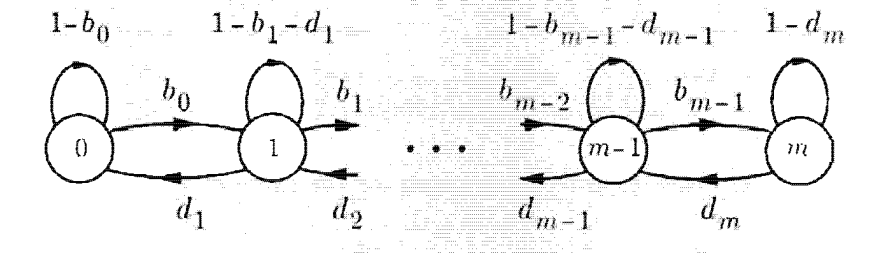
\includegraphics[width=.6\textwidth]{images/P_Markov_Birth_Death.png}
   \caption{Transition probability graph for a birth-death process}
\end{figure}

For two neighboring states $i, i+1$. For another transition of $i \to i+1$ can occur there must a transition of $i+1 \to i$. Therefore expected frequency of transitions satisfies
\[\pi_i b_i=\pi_{i+1}d_{i+1}, \quad i=0,1,\ldots,m-1\]
This leads us to local balance equations
\begin{align*}
    \pi_i &= \pi_0 \frac{b_0 b_1 \cdots b_{i-1}}{d_1 d_2 d_i}, \quad i=1,2,\cdots, m \\
    \sum_i \pi_i &= 1
\end{align*}

\begin{remark}
    Consider the case where $m$ is very large and $b>d$ the steady state probability of all states will be zero and it will be transient. Thus even with aperiodic single recurrent class a \MC{} may fail to reach steady state values and a steady-state distribution may not exist.
\end{remark}
\part {Geometry}
\part {Linear Algebra}
\chapter{Introduction}

The heart of linear algebra is in two operations-both with vectors.
\begin{enumerate}
  \item add vectors to get $\textbf v + \textbf w$
  \item multiply them by numbers $c$ and $d$ to get $c \textbf v$ and $d \textbf w$
\end{enumerate}
Combining those two operations gives the \textbf{linear combination} $c\textbf v + d \textbf w$.

\section{Vectors and Linear Combinations}

For two matrix $\textbf A$, $\textbf B$ and a scalar $c$

\begin{align*}
  \textbf A &= \begin{bmatrix} x_1 \\ y_1 \end{bmatrix} \\ 
  \textbf B &= \begin{bmatrix} x_2 \\ y_2 \end{bmatrix} \\
  \textbf A + \textbf B &= \begin{bmatrix} x_1 + x_2 \\ y_1 + y_2 \end{bmatrix} \\
  \textbf A - \textbf B &= \begin{bmatrix} x_1 - x_2 \\ y_1 - y_2 \end{bmatrix} \\
  c \textbf A &= \begin{bmatrix} c x_1 \\ c y_1 \end{bmatrix}
\end{align*}





\chapter{Eigenvalue and Eigenvector}

For a square matrix $A$ and a vector $x$ if
\[
  Ax = \lambda x
\]
then the resulting vector $Ax$ is in the same direction as $x$. This vector is called eigenvector and $\lambda$ is called eigenvalue.



% ----------------ADDING IMAGES -------------
%\begin{figure}[!h]
%    \centering
%    \includegraphics[width=.8\textwidth]{}
%    \caption{}
%\end{figure}

\bibliography{cite}
\bibliographystyle{unsrt}
\end{document}
